% !TEX root = tese.tex


A iniciativa Audio Commons visa trazer conteúdo sonoro em Creative Commons (CC) para artistas e indústrias criativas. Licenças CC fornecem uma maneira padronizada para dar permissão ao público no compartilhamento e utilização de trabalho criativo em condições definidas pelos criadores de conteúdo, que pesquisa formas de aproveitamento e utilização de serviços online de distribuição de conteúdo sonoro com licenças em Creative Commons \footnote{\url{https://creativecommons.org/}}. O projeto é financiado pela união Européia e tem entre seus objetivos, desenvolver uma ontologia para sons, e criar um mecanismo mediador para pesquisar sons de diversas fontes como as bibliotecas Freesound.org, um grande repositório de samples; Europeana.org, que reúne um acervo de gravações históricas de diversas instituições européias e Jamendo.com, que reúne músicas novas produzidas em licenças livres.

\subsection{Motivações}
Nosso principal domínio de aplicação é a improvisação musical que é definida como uma atividade musical autônoma \footnote{\cite{Canonne2016}} que geralmente leva a situações pluralistas, com ênfase no processo de tocar, e na iteração musical no momento \footnote{\cite{BERGSTROEM-NIELSEN2016}}. Em oposição à improvisação idiomática, como aquela praticada em algumas formas de jazz ou hip-hop, a improvisação livre pode levar à formas não metrificadas e sem escala ou tonalidade pré-determinadas, onde muitas vezes a variação de timbre prevalece\footnote{\cite{Barthet:11a}}. Já vinha desenvolvendo atividades em improvisação livre anteriormente, mas depois do início do doutorado, tive oportunidade de participar da Orquestra Errante, grupo conduzido pelo professor Rogério Costa que ensaia semanalmente no estúdio do NuSom na Universidade de São Paulo. 

\begin{figure}
   
       %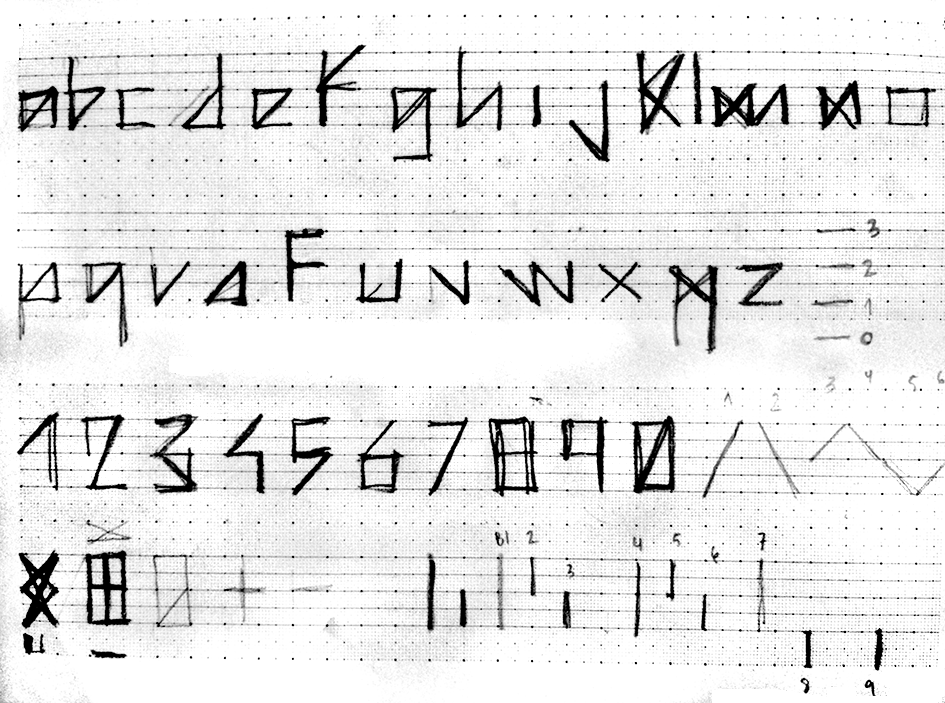
\includegraphics[width=1\linewidth]{pictures/audiotype_sketch}
   \caption{Apresentação do grupo Orquestra Errante.}
    \label{fig:oe}
 \end{figure}

 \chapter{Playsound}
\label{ch:playsound}


\section{Playsound.space}

O desenvolvimento da plataforma Playsound.space (PS) começou durante o meu período de estágio no Centre for Digital Music (C4DM) na Queen Mary University of London (QMUL)\footnote{O Estágio aconteceu de junho de 2017 a maio de 2018 e foi financiado pelo Programa de Doutorado Sanduíche da CAPES}, onde tive a oportunidade de participar do grupo de pesquisa ligado ao projeto Audio Commons\footnote{\cite{Font2016}}. Depois de desenvolver o projeto Banda Aberta, o desejo era de trabalhar no desenvolvimento de um sistema que pudesse ser utilizado como um instrumento musical, que fosse capaz de produzir uma gama rica de sonoridades e não mais somente uma plataforma para tocar sons pré determinados. 



Durante as práticas de improvisação musical que participei até agora, encontrava algumas dificuldades em utilizar softwares tradicionais como DAW ou \emph{patchers}. Uma delas é de que muitos softwares do tipo DAW são baseados em grids temporais fixos, ou seja, existe um tempo que determina o fluxo dos acontecimentos sonoros, e embora esse tempo possa ser mudado, a estrutura rígida conflita com a necessidade da liberdade na improvisação. A estrutura em grade ou se impõe para os demais músicos, como um metrônomo, ou entra em conflito com os demais participantes. Além disso, as estruturas temporais também dificultam a criação de polirritmias. 


Softwares que se comportam como instrumentos virtuais, por outro lado, como sintetizadores e \emph{samplers} são mais fáceis de serem empregados na prática. Por serem baseados em gesto, o controle do fluxo sonoro fica a cargo do musicista, dependendo aí do tipo de controlador que ele usa, de sua expertise técnica em tocar, e da capacidade de variação timbrística do instrumento. No caso dos sintetizadores, as possibilidades de variação de sonoridade são constritas pelos timbres oferecidos pelo fabricante ou programador, e em geral restritas a sons musicais, dentro de uma escala pré-determinada. Além disso, para se obter um bom controle de dinâmica, é recomendado a utilização de controladores externos, como teclados MIDI, por exemplo. Minha idéia era desenvolver algo que pudesse ser tocado em tempo real, e que permitisse mais variação sonora do que os softwares e ferramentas disponíveis no mercado.

No contexto de novas interfaces para produção musical uma série de abordagens diferente têm sido desenvolvidas para o emprego do computador como instrumento musical na prática de improvisação livre. Exemplos incluem \emph{live coding} \footnote{\cite{freeman2011collaborative}} e orquestras de laptop\footnote{\cite{Albert2012}}. \emph{Live Coding} colaborativo ao vivo frequentemente envolve o desenvolvimento de tecnologia para sincronização entre dispositivos\footnote{\cite{Wilson2014}}, que aqui não foi adotada devido à escolha estética de deixar a estrutura rítmica livre.


\subsection{Re-aproveitamento de sons}

A ideia de tocar com uma ``paleta de sons expandida'' tem sido explorada na música desde Luigi Russolo\footnote{\cite{Merz2013}} e especialmente depois da música concreta. Em 1952, Pierre Schaeffer em carta para Pierre Boulez relata sobre a dificuldade de tocar música concreta com intrumentos tradicionais: 

\begin{citacao}
There is no instrument to play concrete music. This is the biggest difficulty. Or else, it is necessary to imagine an enormous machine, of the cybernetic type, capable to perform millions of combinations, but we have not yet got there. So long as I have only two or three record players to realize approximative chains, I shall remain trapped in a discontinuous style where everything seemsto have been hacked out. Is there a compromise? (Scheffer, 1952 in Palombini \citeyear{Palombini1993})
\end{citacao}

Esse dispositivo que seria capaz de realiza múltiplas compinações hoje está acessível a uma parcela considerável da população. Somado isso à digitalização e a disponibilização de sons online potencializa essa ideia, como aponta Schnell:

\begin{citacao}
In the age of digital sound databases and online music publishing services, the total disembodiment of digital sound turns into the promise of perpetual reincarnation of digital sounds through their permanent exchange and transformation.\cite{Schnell2013}
\end{citacao}

Nos instrumentos que funcionam a base de amostras de sons (samplers), as potencialidades sonoras são ampliadas pela possibilidade de utilização de sons não-musicais, ou em outras escalas, mas são dependes de se ter acesso e conhecimento de uma biblioteca grande de sons. 

O músico Kutiman, no álbum \emph{Tru-you} \citeyear{Kutiman2010}, utiliza trechos de diversos vídeos, na maioria vídeos demonstrativos de instrumentos ou técnicas musicais como fonte para a criação de diversas faixas musicais. O trabalho de pesquisa, recorte e montagem é um trabalho tradicional de composição, amparado por softwares de edição de vídeo\footnote{Disponível em: \url{http://thru-you.com/}}. 


\begin{figure}
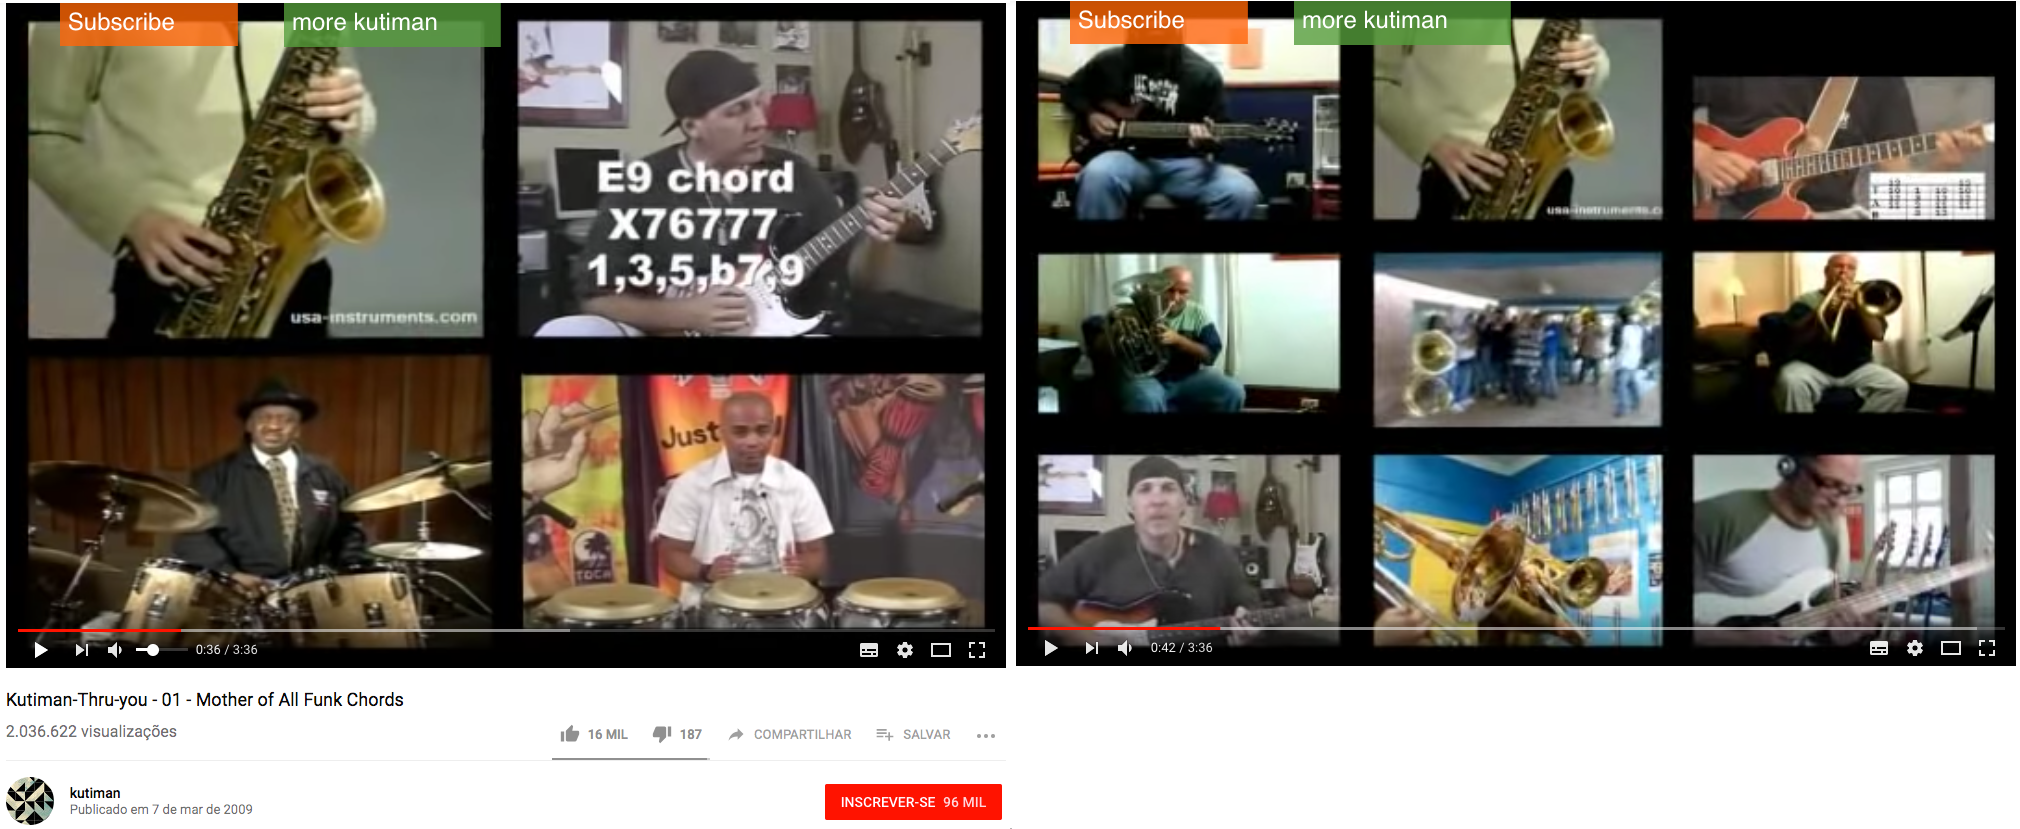
\includegraphics[width=1\textwidth]{pictures/cap4/kutiman}
\caption{Screenshots da faixa ``Mother of All Funk Chords'' do compositor Kutiman. }
\label{Kutiman}
\end{figure}


Localizar samples em tempo real durante uma improvisação musical pode ser desafiador\footnote{\cite{Xambo2018}}, principalmente porque a improvisação exige da musicista uma reação espontânea e instantânea em tempo real \footnote{\cite{canonne2011model}}. Isso exige que a performer conheça bem e previamente os sons de uma determinada coleção, o que se torna impraticável se a coleção de sons é muito grande. Para contornar este problema, praticantes normalmente selecionam uma amostra reduzida de sons, o que acaba também por reduzir suas possibilidades criativas durante as performances.

%A digitalização do som, em conjunto com tecnologias Web e bancos de dados de áudio digital abre muitas possibilidades criativas, que como Schnell aponta, pode levar à ``promessa de reencarnação perpétua de sons digitais através da sua permanente troca e transformação'' \footnote{\cite{Schnell2013}}. 

A utilização de amostras de sons pré-gravados é largamente empregada em uma série de tradições estéticas musicais como no emph{Hip Hop, Plunderphonics, Música Eletrônica, Música Concreta, composição de Paisagens Sonoras}. Bibliotecas online de áudio como Freesound.org, Redpanal.org, Sampleswap.org entre outras são utilizadas por compositores e produtores musicais de vários tipos de aplicações multimídia como cinema, publicidade, video games, e composições musicais \footnote{\cite{Roma2013}}. 

Alguns projetos desenvolvidos recentemente têm também esse norte como paradigma. O projeto API Cultor, por exemplo \footnote{\cite{Ordiales2017}} usa técnicas de \emph{machine learning} para prover um ambiente para re-utilização de sons de blibliotecas online. Lee et al. propõe uma ferramenta para \emph{live coding} com a API do Youtube para improvisação livre \footnote{\cite{Lee}}. Ao prover acesso a seu banco de dados por uma REST API \footnote{\cite{Akkermans2011}}, o site Freesound.org permite que musicistas e designers criem aplicativos que explorem seu conteúdo online para utilização ao vivo. BeatPush \footnote{\cite{Feenstra2016}}, é um exemplo de sequenciador usando esta API e o Freesound Explorer \footnote{\cite{Font2016}}, por exemplo, organiza os sons em uma configuração espacial por similaridade e usa cores para representar aspectos timbrais, no entanto, é uma aplicação mais voltada para navegação e exploração do que para tocar em tempo real, e não permite que os usuários selecionem sons a partir de buscas múltiplas. 
Arne Eingenfeld, do Metacration Lab usa o Freesound como base para produzir música generativa a partir de algoritmos computacionais na peça Coming Together - Freesound\footnote{Vídeo da peça pode ser visto em: \url{https://www.youtube.com/watch?v=jFD2A8bX8TM}}

\begin{citacao}
An autonomous soundscape composition created by four autonomous artificial agents. Agents choose sounds from a large pre- analyzed database of soundscape recordings (from freesound.org), based upon their spectral content and metadata tags. Agents analyze, in realtime, other agent's audio, and attempt to avoid dominant spectral areas of other agents, selecting sounds that do not mask one another. Furthermore, selections from the database are constrained by metadata tags describing the sounds. Thus, water sounds may trigger other water sounds, or agents can choose to oppose contextual references. As the composition progresses, convergence is further facilitated by lowering the bandwidth of the agent's resonant filters, projecting an artificial harmonic field upon the recordings that are derived from the spectral content of the recordings themselves. Finally, each agent adds granulated instrumental tones at the resonant frequencies, thereby completing the ``coming together''. \cite{Arneeigenfeldt2010}
\end{citacao}

Entre diversos serviços que provém conteúdo sonoro online, uma imensa gama de sons musicais e não musicais são oferecidos pelo Audio Commons Ecossystem \footnote{\cite{Font2015}}. A ideia no desenvolvimento do Playsound era de ser uma tentativa de contornar essas questões, promovendo o acesso a esses sons em tempo real através da API do Freesound \footnote{\cite{Akkermans2011}}, oferecendo feedback visual através de espectrográficos, de uma forma que pudesse ser tocada sem um grid de tempo fixo e por usuários sem domínio de técnicas musicais.


\subsection{Motivações}

Compor a partir de espectrogramas era uma ideia que acompanhava meu trabalho já faz algum tempo. Em 2011 publiquei um trabalho chamado UTOPIA (Figura \ref{utopia}), onde desenhava a palavra utopia através de síntese subtrativa sobre uma gravação feita de uma serra de fita em funcionamento, que era uma amostra bastante saturada. Essa ideia também voltou outras vezes no meu trabalho, na composição da peça Bandas Críticas e no processo de composição de sons para o Banda Aberta. 

Espectrogramas (ou sonogramas) são imagens geradas a partir da análise do som por um algoritmo chamado de \emph{Fast Fourier Transform} (FFT), que decompõe as frequências formantes de ondas complexas\footnote{\cite[55]{Roads}}. Diferente da representação da forma de onda, que é a mais comum em softwares de edição de áudio eletrônico, e é uma representação bi-dimensional, onde estão representadas intensidade e tempo de um som, os espectrogramas trazem uma representação que ``incorpora todas as três dimensões do som'' \footnote{\cite{Schafer2011}}, intensidade, frequência e tempo. 


Quando começamos a publicar os primeiros artigos a respeito do projeto Banda Aberta comecei a buscar ferramentas para conseguir imprimir os conjuntos de samples (ver figuras \ref{samplesgalaxias}, \ref{samplespercussao}, \ref{samplescolab} e \ref{samplesorquestra}) e não consegui encontrar nenhuma ferramenta pronta que pudesse gerar espectrogramas de um conjunto grande de sons que fosse acessível. Então, para gerar essas imagens, bem como os sites que reúnem os samples do projeto Banda Aberta, tivemos que desenvolver uma ferramenta própria, que chamamos de ``Spectrogram player'', que foi o esboço de um player para tocar a partir de espectrogramas, em JavaScript e HTML \footnote{A ferramenta foi desenvolvida em código aberto e está disponível no endereço: \url{https://github.com/arianestolfi/spectrogramplayer}}. 

Quando comecei a desenvolver este novo projeto, descobri que a API do Freesound\footnote{\cite{Akkermans2011}} já fornecia os espectrogramas dos sons de sua biblioteca em forma de imagens, o que era muito conveniente para o projeto, já que diminui o tempo necessário para a análise via FFT que poderia gerar os espectrogramas em tempo real. Além disso, ao oferecer os espectrogramas como imagens, a API do Freesound permite realizar a pesquisa sonora sem a necessidade de baixar os sons toda vez no computador do usuário.

\begin{figure}
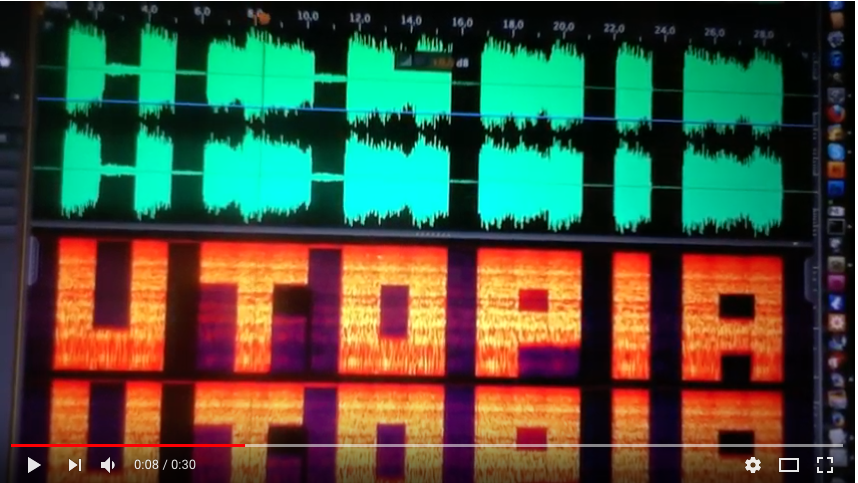
\includegraphics[width=1\textwidth]{pictures/cap4/utopia}
\caption{\label{utopia}Utopia }
\label{utopia}
\end{figure}

Queria desenvolver uma ferramenta que não dependesse de expertise técnica ou virtuosismo, que é um dos objetivos dessa pesquisa. Assim como no projeto Banda Aberta, decidimos manter o texto como forma de interação com o sistema, mas ao invés de fazer um mapeamento de sons por letras, como no projeto anterior, aqui o texto serve como fonte para buscar informações, ao permitir a busca através de significados semânticos ou descritivos, por exemplo: ``chuva pacífica'', ``crowd noise'' ou ``applause''. A solução técnica foi o desenvolvimento de um sistema de busca e de um tocador que permite o acesso a centenas de milhares de sons em Creative Commons baseada na API do Freesound.


\subsection{Desenvolvimento do Projeto}

Comecei a desenvolver o projeto em Julho de 2018, após apresentar o Banda Aberta em alguns eventos na Europa que descrevi na seção anterior. Estava acompanhando semanalmente as reuniões do projeto AC e imaginei um sistema onde pudesse se buscar os sons através de busca de texto, e escolhê-los pelo espectrograma. A primeira idéia, no entanto, era fazer uma espécie de linha do tempo onde se poderia arrastar os sons e compor no espaço da tela. Quando comecei a desenvolver, ideia de linha do tempo foi substituida pela playlist, para que o sistema não ficasse constrito a uma janela de loop fixo. 

\begin{figure}

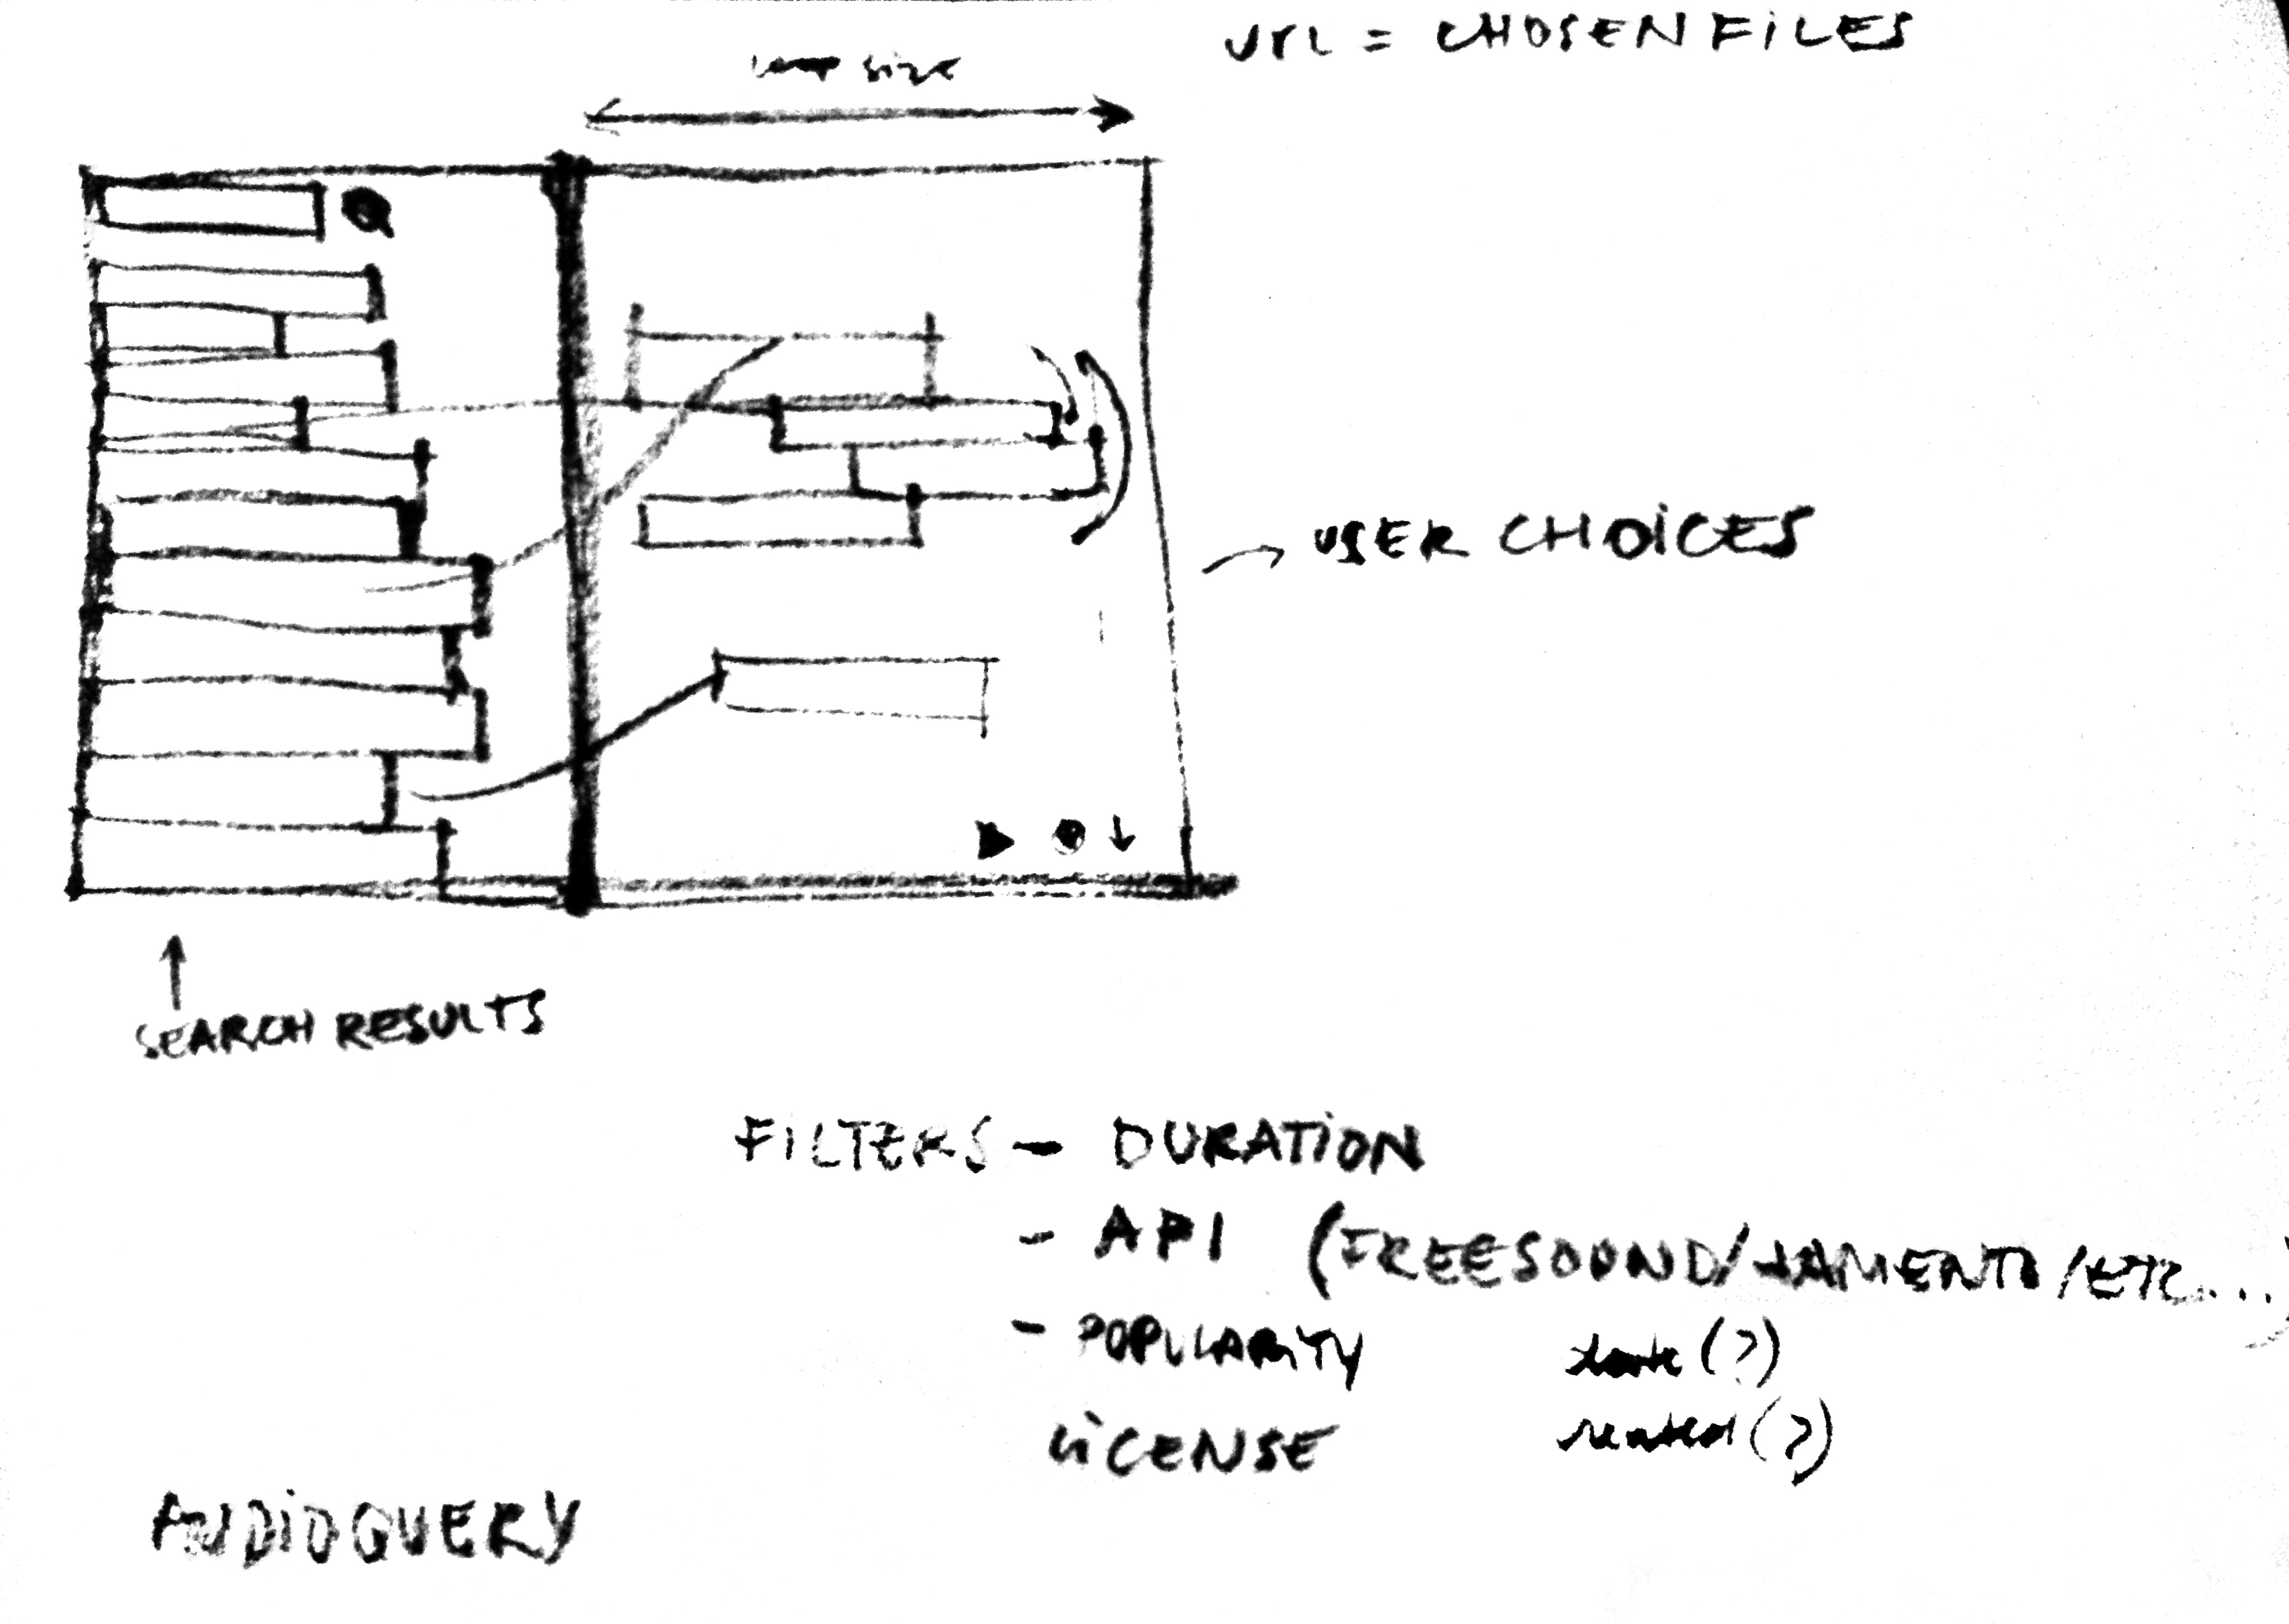
\includegraphics[width=1\textwidth]{pictures/cap4/firstsketch}
\caption{\label{firstsketch}Primeiro rascunho do sistema, que ainda se chamava audioquery}
\label{fig:firstsketch}
\end{figure}


A figura \ref{fig:timeline} apresenta os principais estágios de desenvolvimento da ferramenta de Setembro de 2017 a Julho de 2018. Utilizei novamente Lean Ux \cite{Liikkanen2014} como metodologia de desenvolvimento de software. Dentro dos princípios desse método, começamos novamente o projeto a partir de um protótipo bem simples, que era apenas um sistema de busca que mostrava o resultado como um conjunto de espectrogramas. Inicialmente, contei com a ajuda do programador Miguel Ceriani para fazer a ligação com a API do freesound.

\begin{figure}

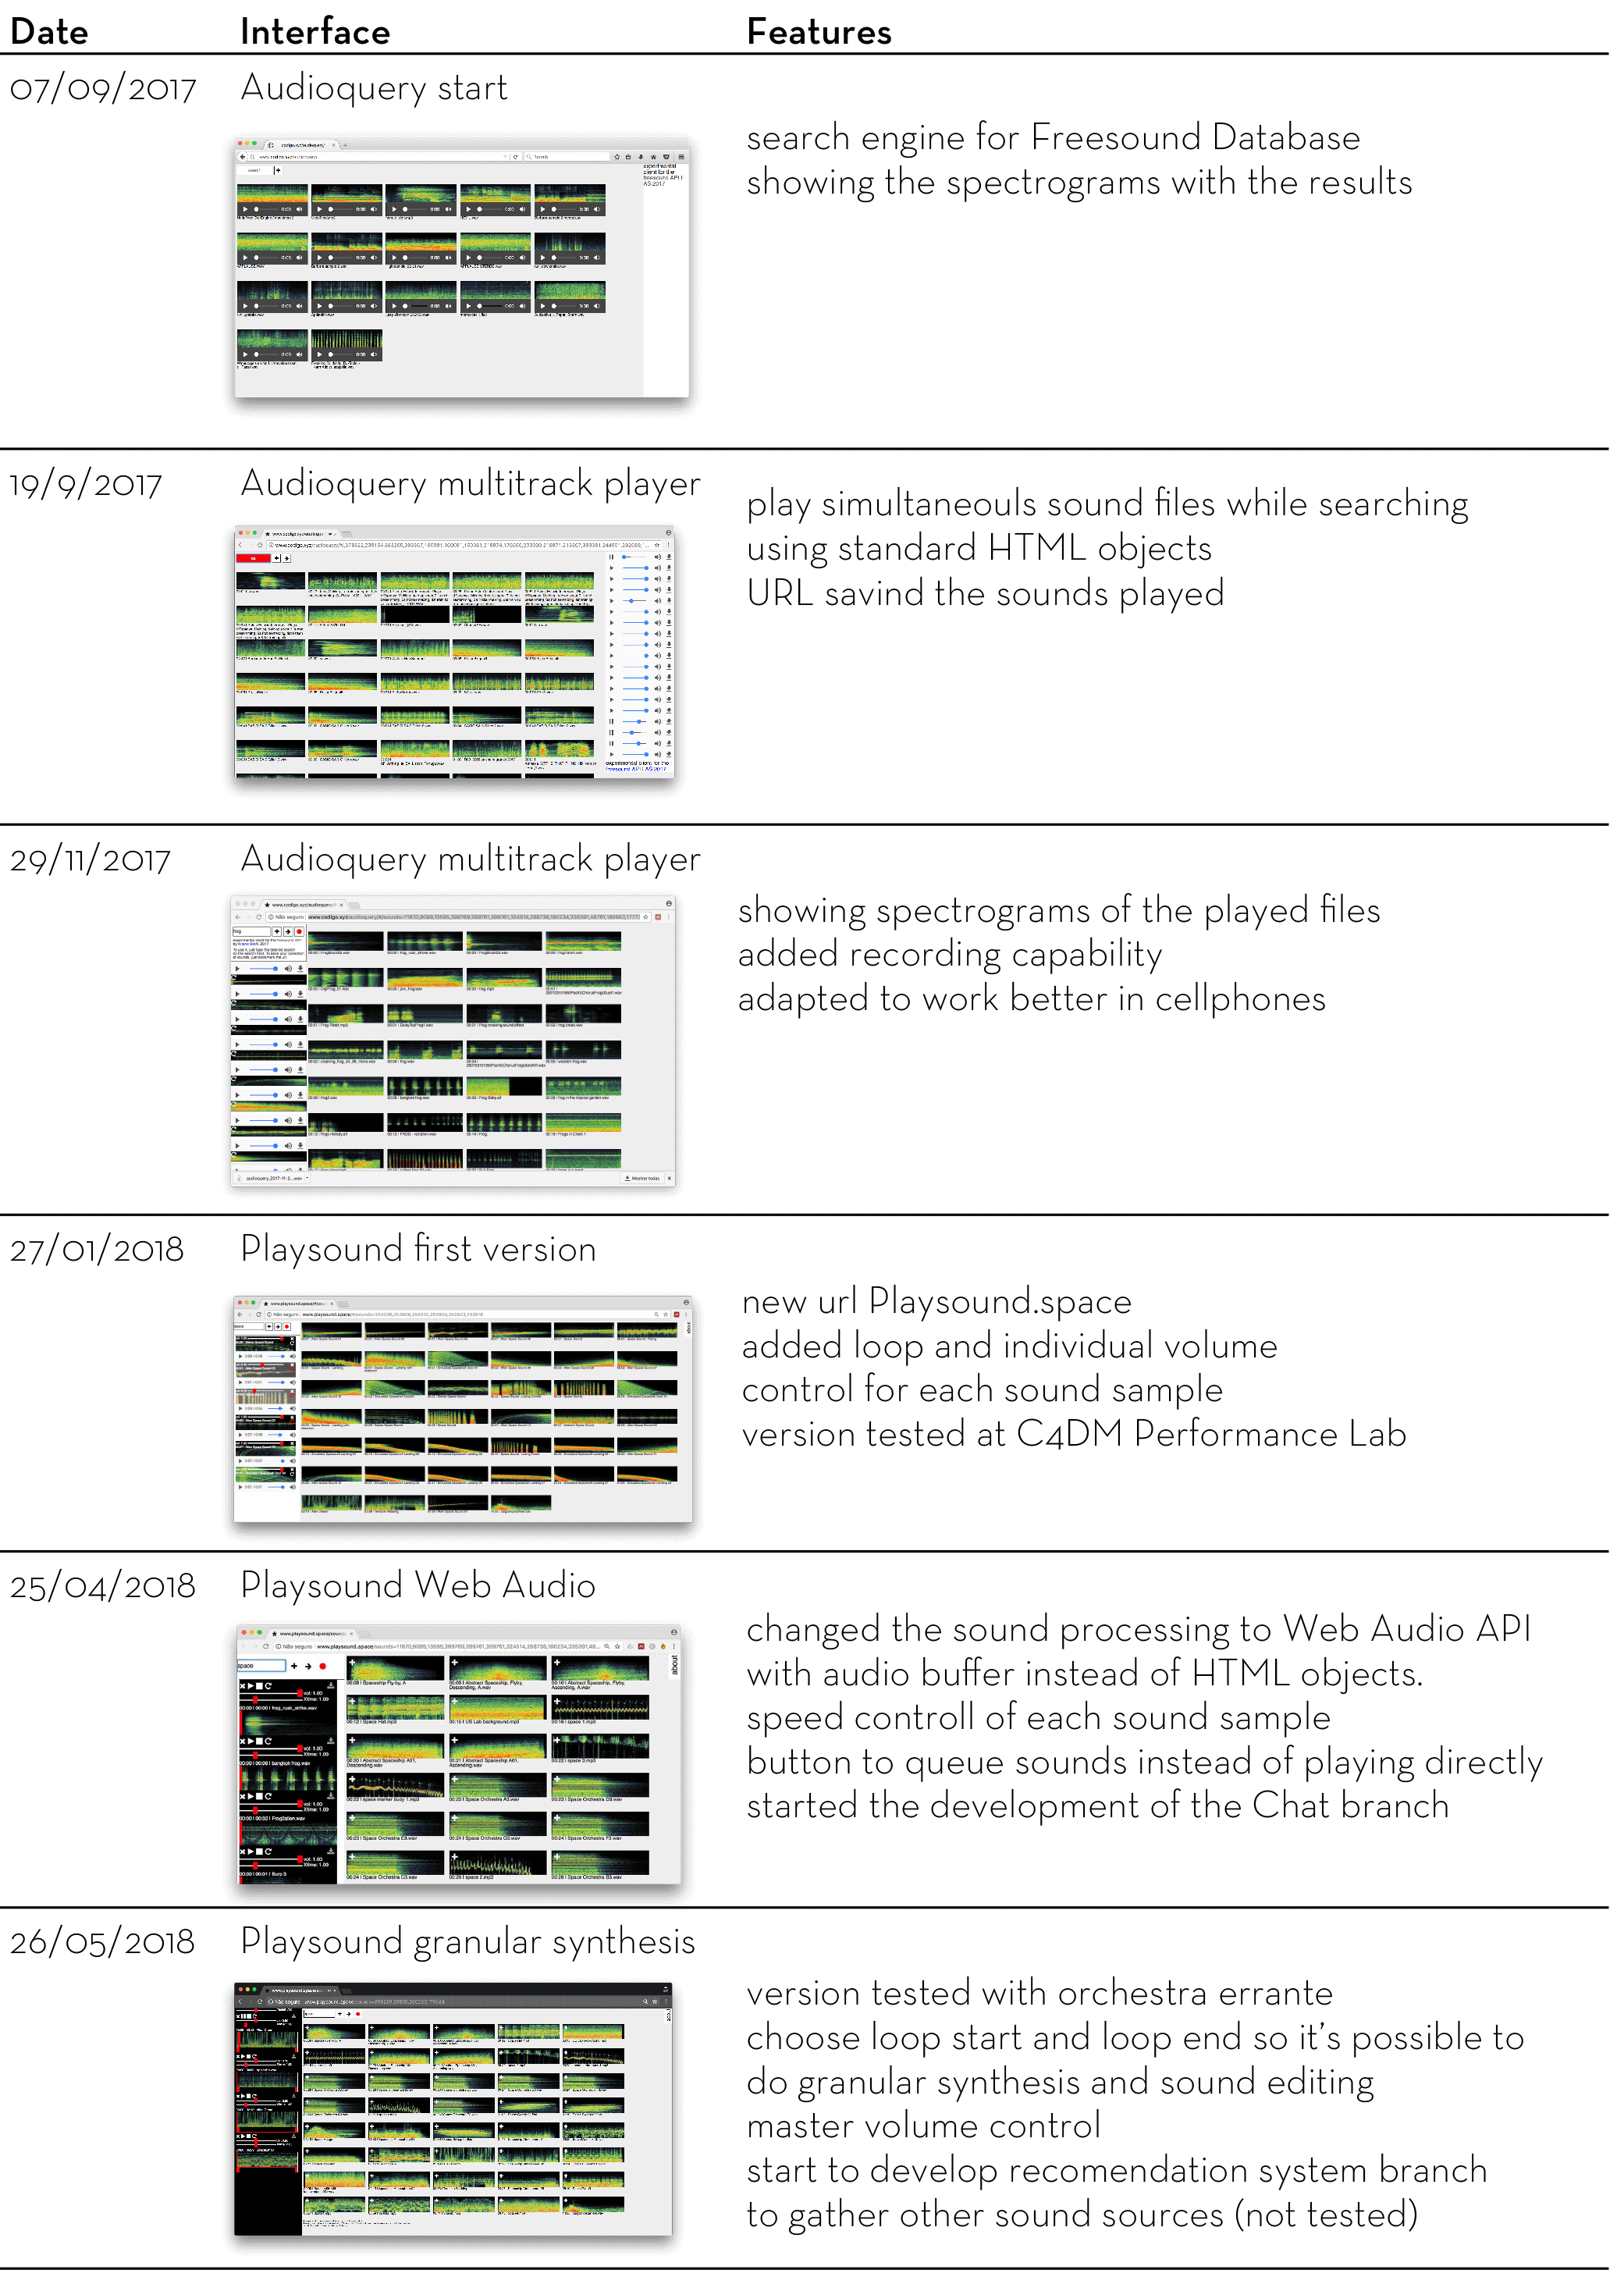
\includegraphics[width=1\textwidth]{pictures/playsoundtimeline}
\caption{\label{pstimeline}Playsound development timeline}
\label{fig:timeline}
\end{figure}

Utilizamos como \emph{framework} Angular.js\footnote{Angular.js é um \emph{framework} em JavaScript desenvolvido pela Google que permite automatizar certos processos computacionais e facilita a comunicação com bancos de dados}. O Framework fornece o recurso de ligação de dados bidirecional, que faz com que a busca aconteça no servidor simultaneamente ao se digitar o texto na caixa de busca. Deste modo, mesmo antes de se completar uma palavra, resultados já começam a aparecer na janela do navegador. Para o processo de improvisação livre, esse recurso se mostrou muito interessante, uma vez que sons não esperados podem surgir mesmo antes de se estabelecer um vocábulo definitivo. O site foi construído como um aplicativo de página única, o que permite com que os conteúdos sejam alterados sem que haja um recarregamento da página\footnote{\cite{Jadhav}}. Assim, a interação dos usuários não interrompe o fluxo sonoro.

Os resultados são apresentados na forma de espectrogramas, que permitem que o usuário do sistema tenha informações sobre ritmo e timbre das amostras recebidas antes de escolher o som para tocar. Aparecem como uma matriz, que permite que se compare os sons visualmente. Apesar de a leitura dos espectrogramas não ser uma coisa corriqueira para qualquer usuário do sistema, acreditamos que um aprendizado implícito pode acontecer no simples processo de pesquisar e tocar com o sistema, quando se percebe a co-relação entre a representação gráfica das propriedades espectro-temporais dos dos sons e suas qualidades audíveis. Quando selecionamos uma imagem, o som é adicionado a uma playlist na lateral da interface.

 Assim que colocamos o sistema no ar, começamos a desenvolver recursos adicionais para transformar o sistema em um instrumento musical de fato. O primeiro recurso desenvolvido foi a capacidade de se fazer novas buscas enquanto os sons são tocados, recurso que já não existe no próprio Freesound. Em seguida, criamos um sistema de url para armazenar uma coleção de sons feita previamente. Cada som selecionado gera um código que fica registrado no endereço do navegador. Desta forma, é possível recuperar uma ``composição de sons'' para utilização futura. O próximo passo foi desenvolver a interface para tocar os arquivos. A primeira versão funcionava baseada em objetos HTML, utilizando o \emph{player} padrão dos navegadores para objetos de áudio que oferece controles apenas de pausar tocar, alterar o instante tocado e dependendo do navegador um controle de volume. Em uma segunda versão utilizamos o tocador do Freesound, que oferecia recursos de loop, mas isso exigia que se recarregasse a página, interrompendo o fluxo musical. 

 Desenvolvemos alguns recursos básicos do tocador, adicionando a imagem do espectro sonoro como recurso mnemônico, e adicionamos controle individual de volume e loop para cada som que era adicionado à playlist. Como recurso de usabilidade, para dar feedback visual, a transparência da imagem é alterada conforme o volume do som aumenta ou abaixa. Adicionamos também um gravador embutido no sistema, que permite que as seções sejam gravadas em arquivos WAV. Esses arquivos podem ser salvos ou re-inseridos na interface para serem tocados. A figura \ref{fig:audioquery} mostra a interface da primeira versão do software no Google Chrome, que até esse momento chamávamos de Audioquery. \footnote{Por questões acadêmicas, mantemos ainda uma versão funcional do software em \url{http://www.codigo.xyz/audioquery/\#/sounds=49333,415849}}.

\begin{figure}

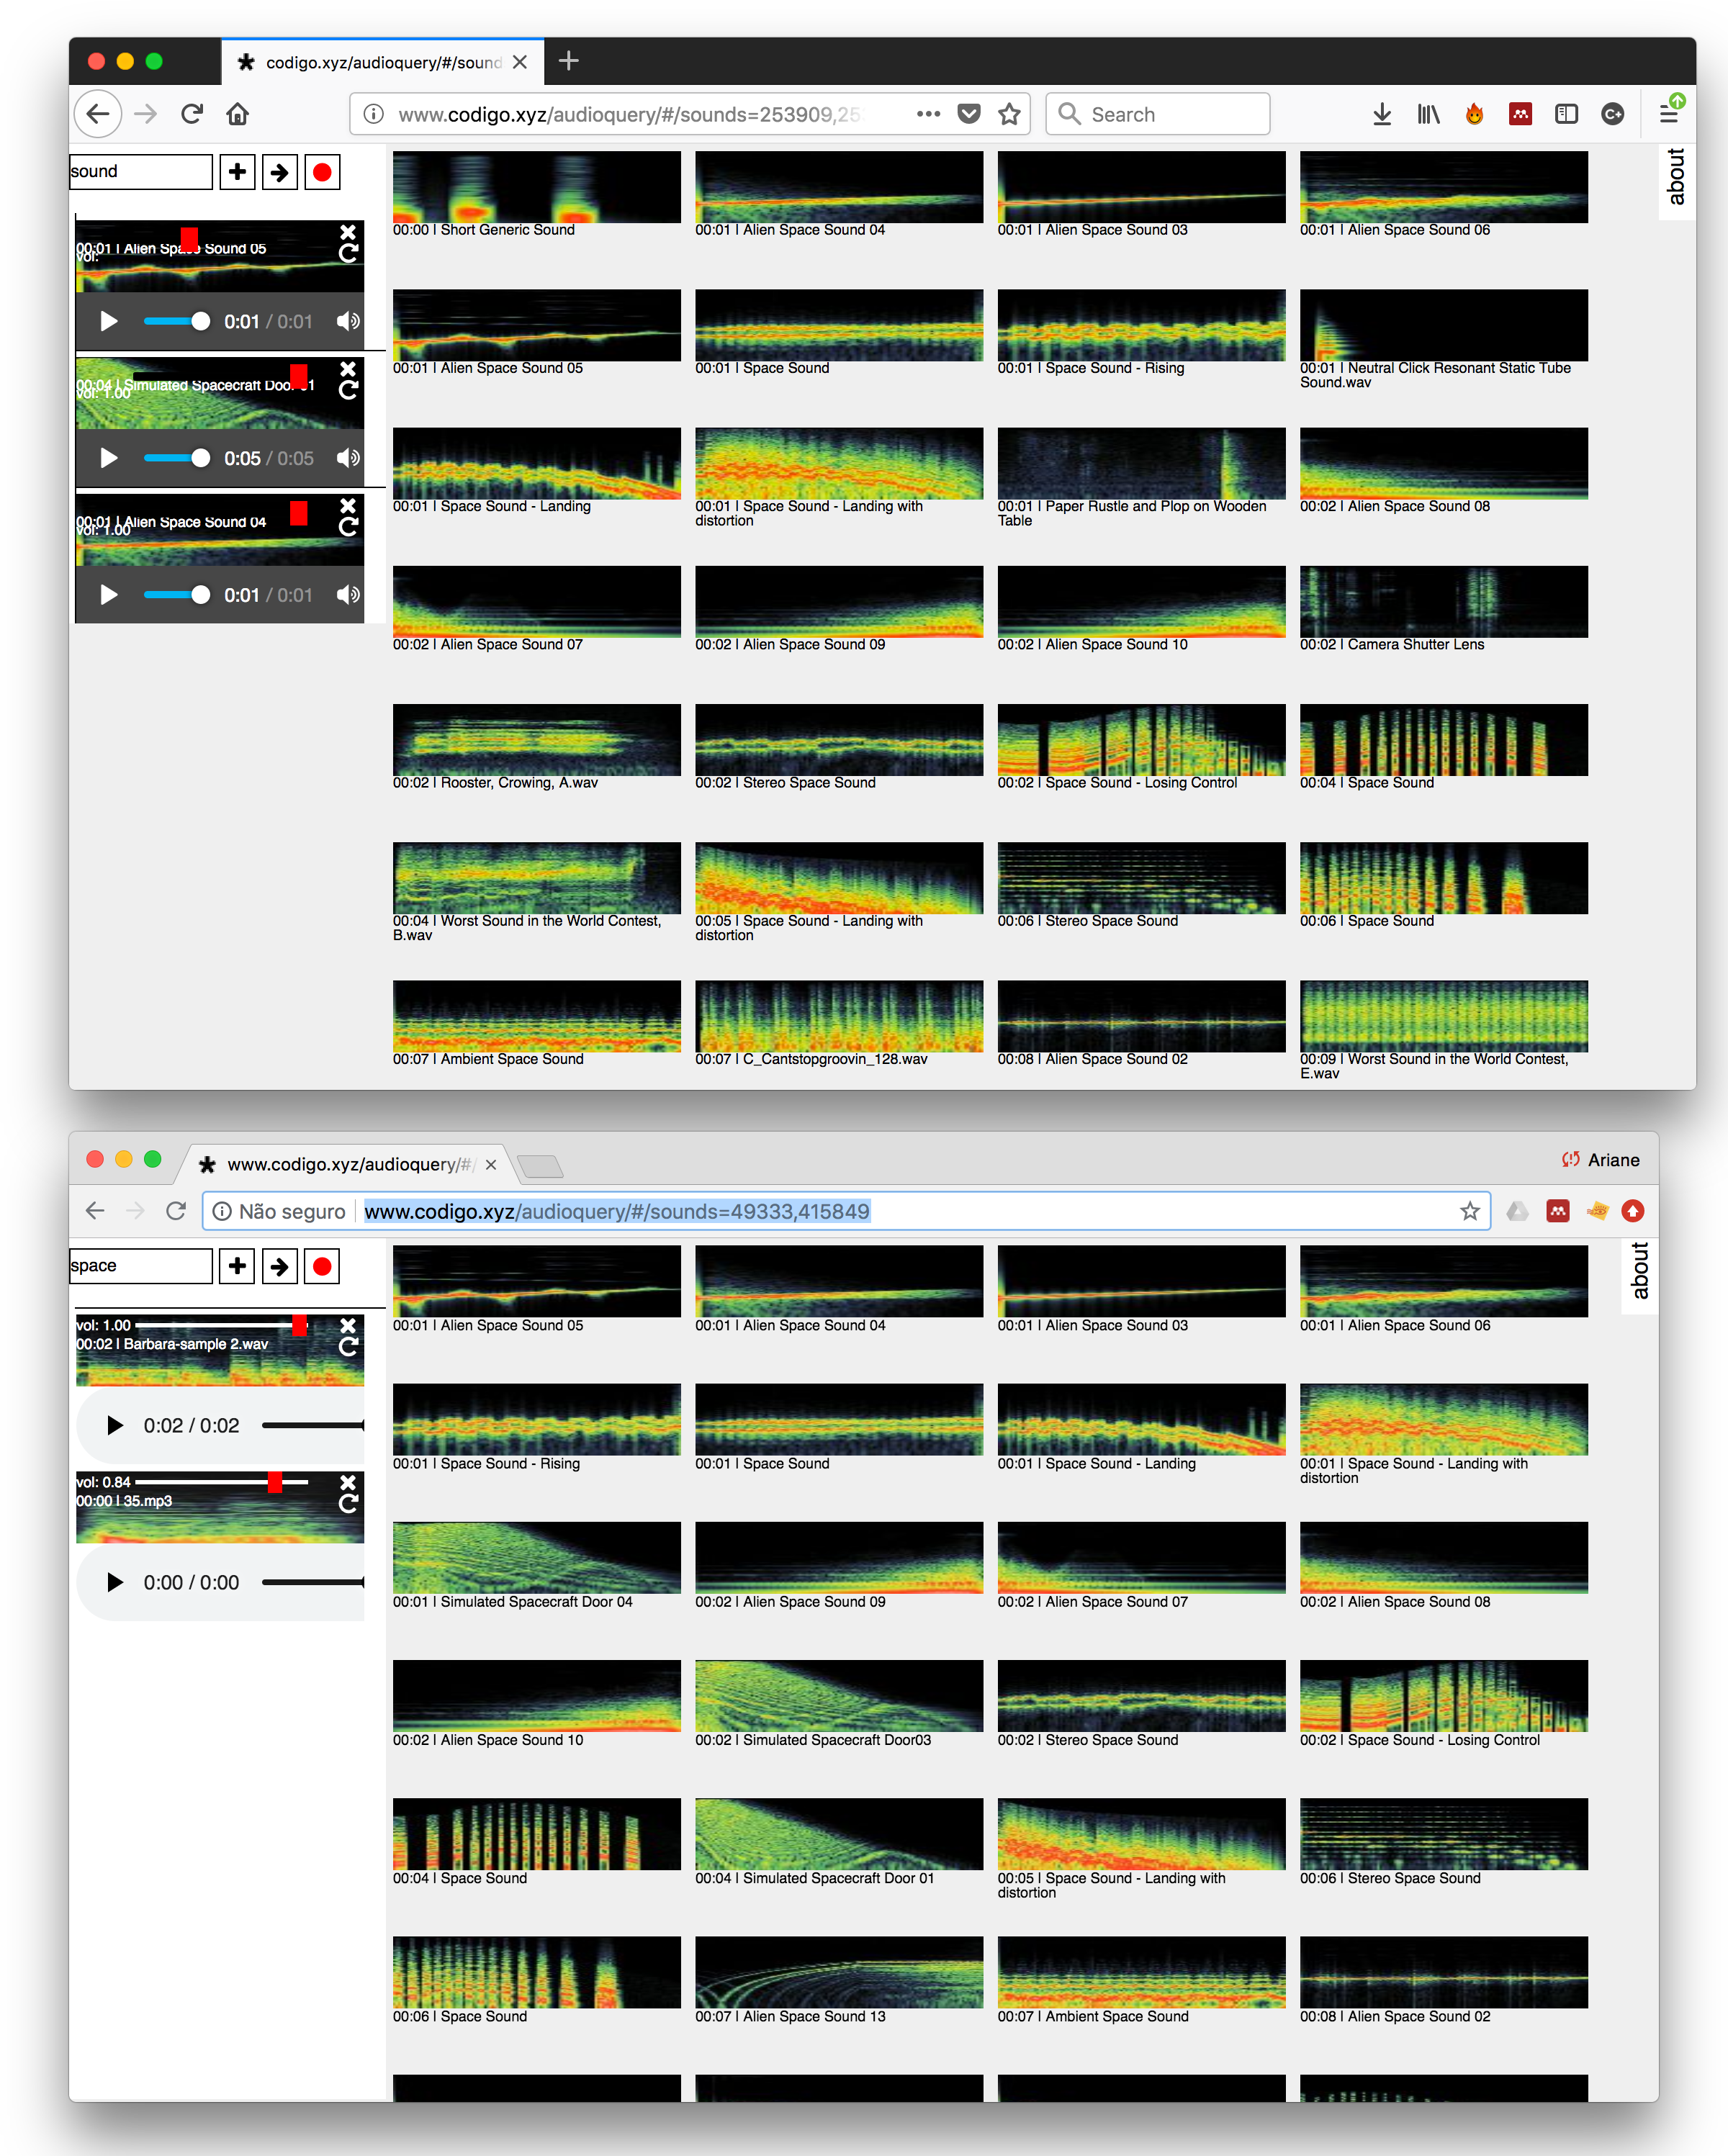
\includegraphics[width=1\textwidth]{pictures/cap4/audioquery_browsers}
\caption{\label{audiquery}Primeira versão funcional do software desenvolvida.}
\label{fig:audioquery}
\end{figure}

\subsection{Primeiras avaliações}

Durante esta primeira fase, as avaliações foram feitas principalmente pela autora, mas também contando com a opinião de alguns colegas convidados para testar informalmente a ferramenta. Esses testes fora de condições de laboratório são previstos dentro de uma perspectiva de metodologias ágeis de programação. A partir desses primeiros testes, pudemos observar informalmente o comportamento de alguns usuários com o sistema e afinar o sistema para realizar testes de usuário mais formais. 

A primeira peça gravada com o sistema chamei de ``spacefrogs''\footnote{Disponível em: https://soundcloud.com/asss/spacefrogs}, foi publicada em novembro de 2017. Foi uma sessão de improviso feita com temática espacial e pântanosas, como qe criando uma atmosfera de ficção científica. Naquele momento, o sistema ainda não contava com controles de volume individuais para cada faixa. Podemos notar pela análise espectral da peça (Ver figura \ref{fig:spacefrogs} e \ref{fig:spacefrogsdt} ) que existe um grande contraste de materiais sonoros, mas pouca variação de dinâmica nos materiais empregados.

\begin{figure}

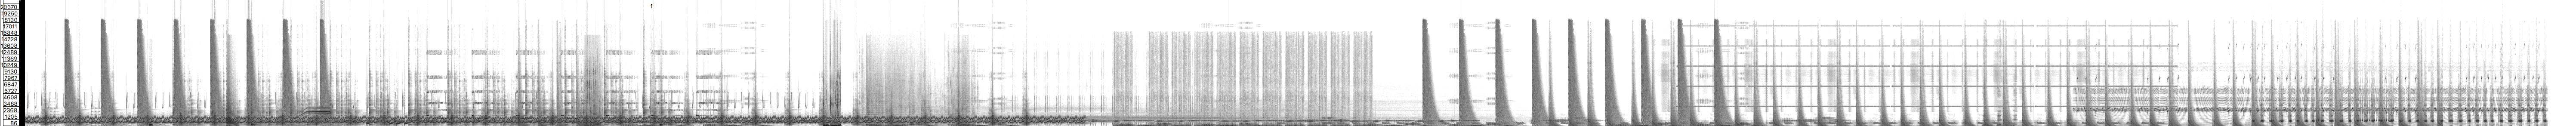
\includegraphics[width=1\textwidth]{pictures/cap4/spacefrogs_spectrogram}
\caption{Espectrogramas da faixa ``spacefrogs''. Gerado pela autora utilizando o software sonic visualiser.}
\label{fig:spacefrogs}
\end{figure}

\begin{figure}

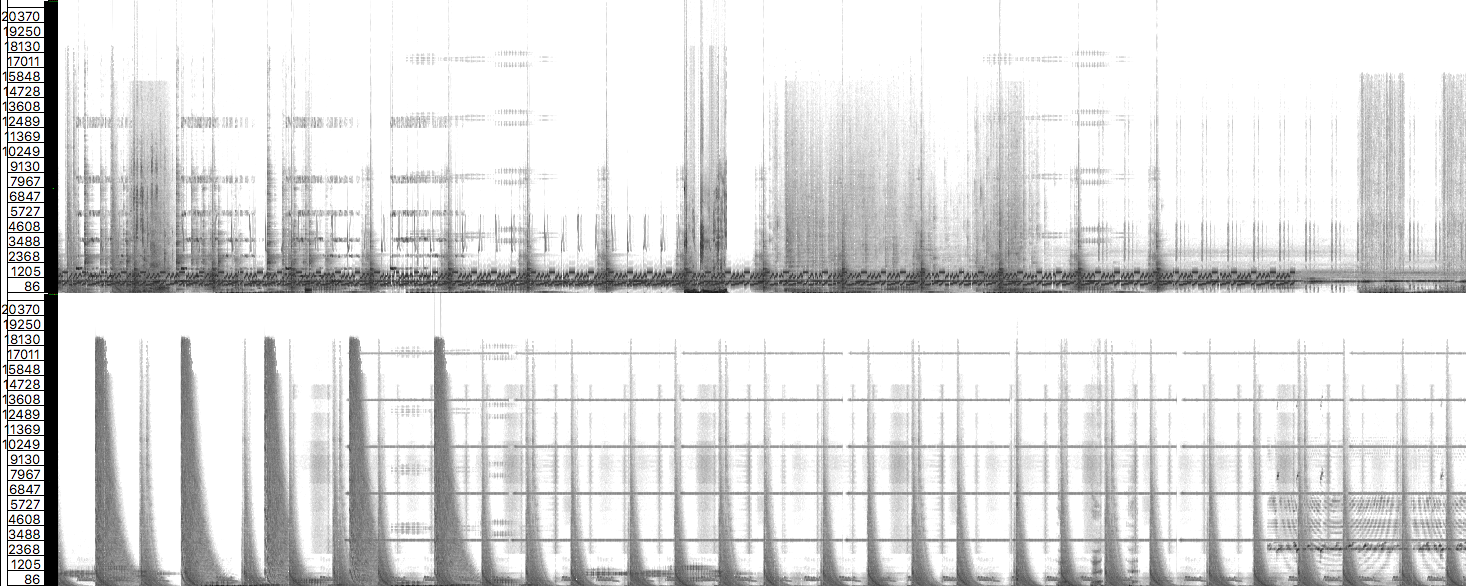
\includegraphics[width=1\textwidth]{pictures/cap4/spacefrogs_spectrogram_dt}
\caption{Detalhes da faixa ``spacefrogs''. Gerado pela autora utilizando o software sonic visualiser.}
\label{fig:spacefrogsdt}
\end{figure}



%Alguns resultados desses testes informais foram gravados, como quando apresentei o sistema para o designer de som 


 %Mais adiante, passei a contar com a ajuda da {}programadora Alessia Millo, que colaborou no desenvolvimento do tocador e de outros recursos que implantamos no sistema. Ela trabalhou na adaptação do sistema para utilizar as tecnologias de Web Audio, ao invés dos objetos HTML, que permitiu uma série de recursos que implementamos posteriormente, como a possibilidade de escolher o começo e o fim dos pontos de loop, alterar a velocidade de reprodução de sons e posição estéreo dos sons.

\subsubsection{Puppets Ensemble}

A partir do ponto que consideramos o sistema satisfatório para ser utilizado em performances ao vivo, (\ref{fig:timeline}), passamos a realizar com ele processos de avaliação mais formais. 

O primeiro deles, foi um processo de avaliação baseado na prática, e para isso, queríamos testar o sistema em condições ``reais'' de uso. Como a principal função do sistema era o de ser empregado em práticas de improvisação livre, montamos um pequeno grupo de improvisação na QMUL, o ``Puppets Ensemble'' para o qual convidamos músicos e interessados dentro do C4DM. Marcamos alguns ensaios, com músicos tocando com o sistema e outros tocando instrumentos tradicionais ou eletrônicos que já praticavam. A proposta desses ensaios, que duraram cerca de uma hora cada e aconteceram no Laboratório de Performance da QMUL, era de tocar algumas sessões de improvisação livre de cerca de 10 minutos e discutir, na sequência de cada sessão, as impressões estéticas e o uso da ferramenta no processo.

Nessas sessões, toquei com Playsound e também com um microfone onde improvisei com a voz. Além disso, participaram Anna Xambó (Supercollider e Playsound), Simin Yang (Playsound), Parham Bahadoran (Percussão e aplicativos de celular). Luca Truchet (Playsound) e Mathieu Barthet (guitarra com efeitos), três mulheres e três homens, com idade média de 33 anos (Ver arranjo na tabela \ref{tab:puppets}). Dos participantes, somente Chen não tinha prática anterior em improvisação musical. Mesmo assim, ela foi capaz de utilizar o sistema sem treinamento anterior.

Com esse processo, pudemos testar se o sistema poderia ser usado de fato como um instrumento musical, e se era possível de ser utilizado em conjunto com outros instrumentos em situações reais de performance. Em todas sessões, tanto quem tocou com a ferramenta quanto os demais musicistas ficaram satisfeitos com as improvisações. Nenhum dos participantes tinham tocado juntos previamente e foi possível estabelecer um diálogo musical durante as sessões. A ferramenta foi elogiada pela riqueza dos sons que provia, Um dos participantes comentou que gostava do fato de que ``qualquer ideia de som que eu tenho eu posso ter nas minhas mãos''. 

O feedback dos usuários também foi importante para notarmos algumas limitações do sistema naquele momento. O primeiro protótipo, não tinha por exemplo o nome dos sons na playlist, o que dificultava o uso para pessoas sem prática de leitura dos espectrogramas. Também não tinha controle individual de volume para cada som, então a possibilidade de controle de dinâmica ainda era muito reduzida, e incluímos melhorias nesse sentido para realizar as próximas rodadas de avaliação.   \footnote{Gravações das seções podem ser encontradas em \url{http://finetanks.com/records/puppets/}}.

\begin{table}

\caption{Performers in music improvisation mixed ensemble sessions: (M): musician; (N): non-musician.}
\begin{tabular}{|lc|} \hline
Sessões & Performers \\ \hline
1 & Ariane (M), Anna (M), Simin (N), Mathieu (M)\\ \hline
2 & Ariane (M), Parham (M), Mathieu (M) \\ \hline
3 & Ariane (M), Simin (N), P4 (M), Mathieu (M), Luca (M)\\
\hline\end{tabular}
\label{tab:puppets}
\end{table}

\subsubsection{Teste com usuários}

Depois desta primeira avaliação prática, passamos a discutir como faríamos uma avaliação mais formal e se isso seria necessário para a publicação de um primeiro artigo científico sobre o uso da ferramenta, que foi publicado na Conferência New Interfaces for Music Expression (NIME) de 2018. Isso gerou um grande debate com meu orientador na QMUL, uma vez que testes de usuário em laboratório poderiam ser contradizentes com a ideia geral norteadora do projeto, que era o desenvolver um software sobretudo para uso pessoal e não necessariamente um produto para o mercado. 


A contradição maior era de que esses testes demorariam muito tempo e a análise dos resultados seria muito complexa, tomando tempo que poderia ser empregado no desenvolvimento e programação do sistema. Por outro lado, uma avaliação formal ou seja, ``que apresente um roteiro estruturado de coleta de dados e resultados'' \footnote{\cite{Stowell}} era importante para o processo, e também para conseguir comparar a ferramenta com outras que estavam sendo desenvolvidas dentro do contexto do projeto Audio Commons, Audio texture, Sample Surfer e o próprio Freesound, para tanto, aplicaríamos um questionário similar ao que já estava sendo utilizado para avaliar essas ferramentas.


Decidimos então fazer o teste mais formal, em condições controladas de laboratório, para o qual convidamos 15 voluntários, com graus diferentes de intimidade com práticas musicais e de improvisação livre (Figura \ref{usertest}). O pesquisador Luca Truchet se dispôs a colaborar na aplicação dos testes e na análise estatística dos resultados obtidas, assim como meu supervisor no C4DM, que fez a análise temática das respostas dos questionários. Nesse momento também, onde começamos a divulgar a ferramenta para o público, passamos a chamar o sistema de Playsound e registramos o domínio onde o site está hospedado.


\begin{figure}

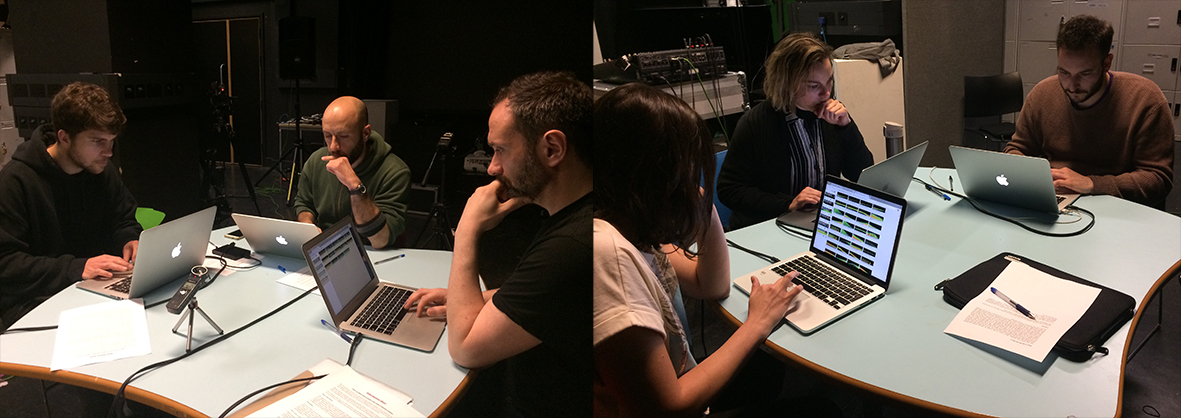
\includegraphics[width=1\textwidth]{pictures/cap4/usertest}
\caption{\label{usertest}Fotos dos testes com usuários no laboratório do C4DM.}
\end{figure}
%When the system was judged ready to be used in live performances (Audioquery multitrack player in Figure \ref{fig:timeline}), we conducted several user evaluations \cite{Stolfi2018b}. First, we established a small ensemble including musicians playing PS and other musicians playing electronic or traditional instruments such as guitar and effects, piano, percussions, and vocals. In each session, participants were invited to play together an improvisation piece for about 10 minutes, and to discuss their experience after each piece. We examined three sessions with this kind of ensemble, involving 6 musicians in total. Following this study, we improved the interface to provide individual volume control and information about the audio file on the playlist.\footnote{Audio recordings of seven 10 min improvisation pieces are available at the link:\url{http://finetanks.com/records/puppets/}}


Existe muita discussão sobre como fazer testes de avaliação de ferramentas para performance musical ao vivo\footnote{\cite{Barbosa2015}}, como aponta Stowell\footnote{\cite{Stowell}}, porque ``interações musicais tem aspectos criativos e afetivos'', que não são fáceis de medir através de tarefas, como é comum no campo do design de interação. Além disso, existe um debate sobre abordagens qualitativas, que são baseadas em relatos sobre a experiência e quantitativas, baseadas em estatísticas e levantamentos quantitativos. Nós decidimos por uma abordagem mista, com aspectos qualitativos e quantitativos.

Como atividade, propusemos aos voluntários, que foram organizados em cinco trios. Inicialmente, os participantes foram brevemente instruídos sobre o funcionamento do sistema, e em seguida convidados para tocar três sessões de improvisação livre. Como o grau de envolvimento dos participantes com esse tipo de prática musical era diferente, dissemos que poderiam tocar o que quisessem, mas que tentassem ouvir o que os outros estavam tocando para compor uma peça coletiva. Após cada sessão de improvisação, discutimos brevemente os resultados estéticos e como a ferramenta influenciou nesses resultados. O final, aplicamos um questionário (Ver Anexo), que incluíam questões sobre o perfil demográfico dos participantes (idade, gênero e experiência musical), de usabilidade (escala SUS de usabilidade\footnote{\cite{Jordan1996}}), questões específicas para medir o suporte à criatividade\footnote{\cite{Cherry2014}} e questões gerais para feedback sobre o sistema. 

As questões de usabilidade foram aplicadas utilizando uma escala Likert de cinco pontos \footnote{A escala Likert é uma escala psicométrica para medir o grau de concordância com determinadas afirmações, indo de discordo totalmente a concordo totalmente, com gradações intermediárias}. Foram incluídas também algumas questões para medir níveis de engajamento, aprendizado, inovação, relevância, qualidade da descoberta dos sons, familiaridade e utilidade dos espectrogramas. Essas questões respondidas em escala Likert foram submetidas a análises estatísticas usando o teste de Mann-Whitney-Wilcoxon, para observarmos também se havia alguma variação significativa na satisfação dos usuários músicos e não músicos.

Quanto à usabilidade e engajamento, não houve diferença significativa entre os resultados obtidos pelos músicos e pelos não-músicos. A Figura \ref{fig:SUS} mostra os resultados obtidos na avaliação de usabilidade. Em geral, os usuários definiram o sistema como fácil de usar, fácil de aprender a usar, conveniente, que não havia necessidade de aprender muita coisa antes do uso, não necessita de suporte técnico para seu uso, que não é um sistema desnecessariamente complexo. Os usuários foram neutros quanto à possibilidade de usar o sistema frequentemente, isso talvez seja relacionado com a tarefa, já que vários usuários não têm perspectivas de práticas em improvisação livre. De um modo geral, o sistema obteve uma nota muito boa seguindo a métrica do sistema SUS (Média = 82.5, Desvio Padrão = 8.94)

\begin{figure}

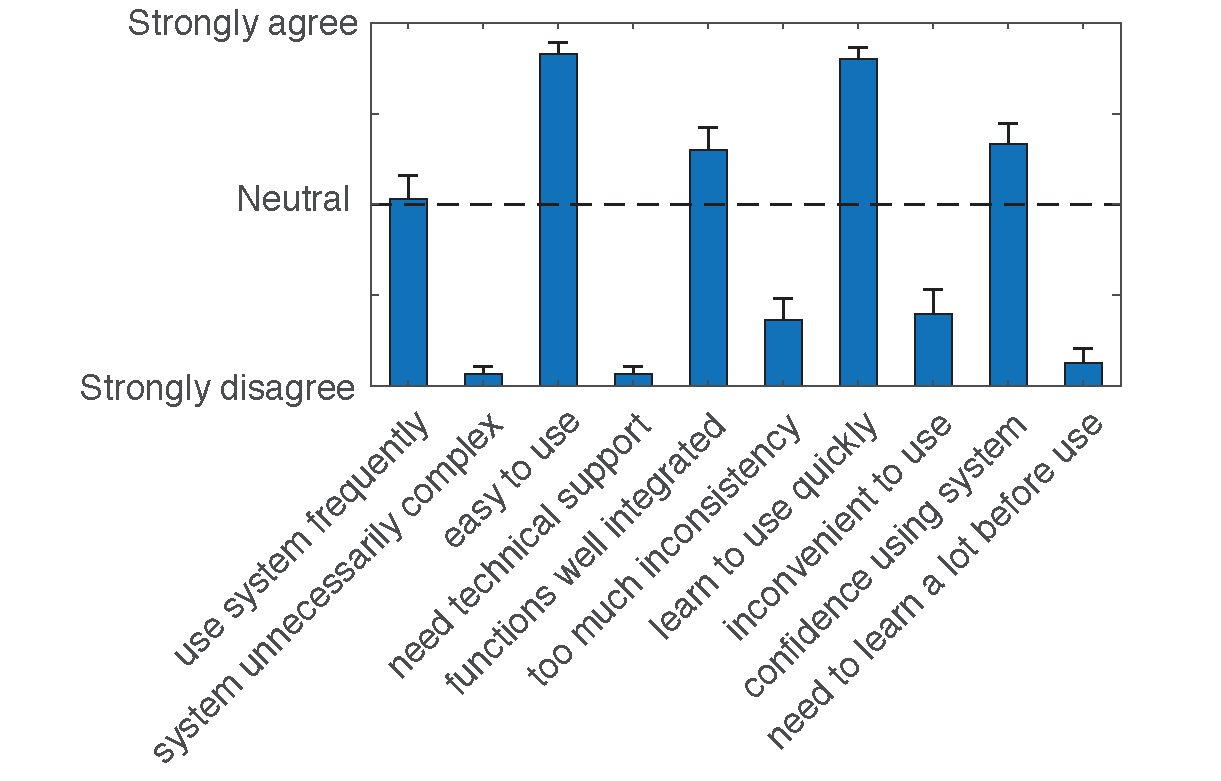
\includegraphics[width=1\textwidth]{pictures/cap4/SUS_lower}
\caption{Resultados obtidos na avaiação de usabiliade.}
\label{fig:SUS}
\end{figure}

Também fizemos uma avaliação quantitativa das respostas dos usuários sobre níveis engajamento, aprendizado e sobre a interface. A figura \ref{fig:questionnaire}, que apresenta os resultados obtidos indica que os participantes se sentiram engajados de uma maneira geral. Quanto à questão a respeito de se os usuários haviam aprendido algo com o instrumento, as respostas foram neutras. Nessa questão as pessoas que tinha mais prática com música também foram as que discordaram mais sobre aprender algo com o software. Os participantes concordaram em média que a forma de compor música usando Playsound era novidade para eles, e tiveram diferentes graus de dificuldade para encontrar os sons que esperavam durante as sessões. 

Quanto à familiaridade com o uso de espectrogramas, tivemos também um resultado neutro, uma vez que a maioria dos participantes tinha familiaridade e o restante não. Também foi neutro o resultado a respeito da utilidade do uso dos espectrogramas, que variou de acordo com a familiaridade dos usuários.


\begin{figure}

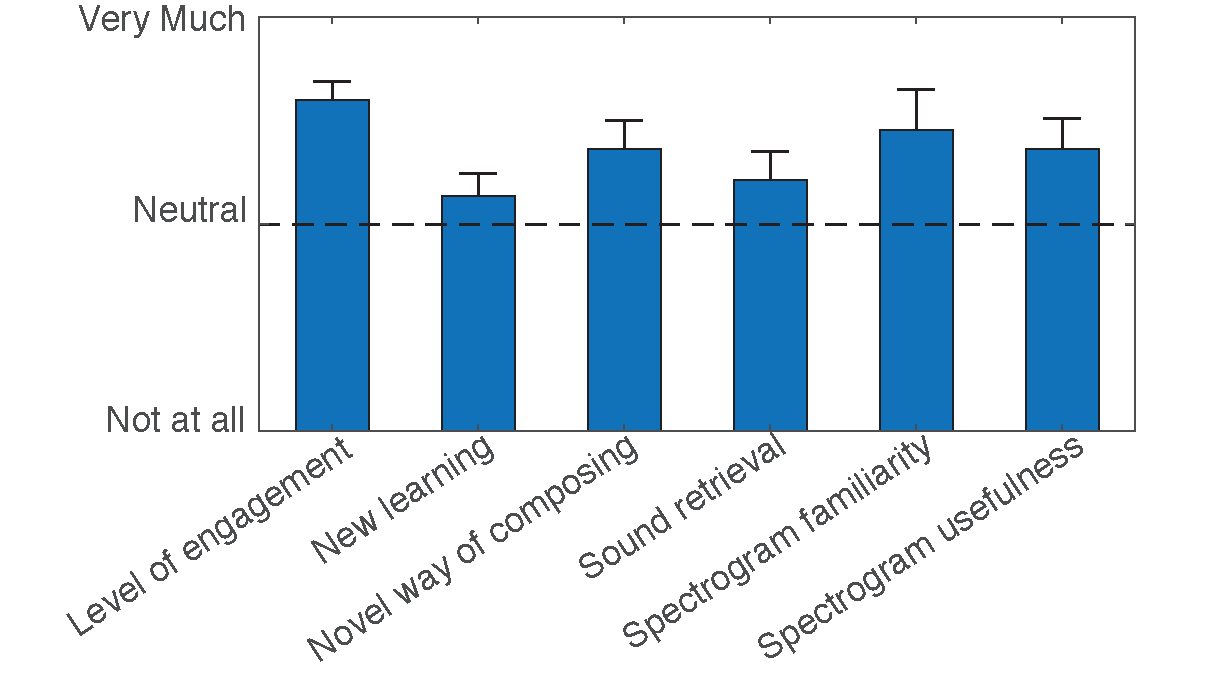
\includegraphics[width=1\textwidth]{pictures/cap4/questionnaire_lower}
\caption{\label{amas}Resultados obtidos na avaiação do questionário.}
\label{fig:questionnaire}
\end{figure}

Uma segunda parte do questionário incluiu questões relativas à medição do índice de suporte à criatividade (CSI). O método\footnote{\cite{Cherry2014}}, descitro por Cherry inclui um questionário psicométrico que busca testar a capacidade de uma ferramenta para dar suporte aos processos criativos de seus usuários. Para isso, apresenta algumas questões a respeito do desempenho em quesitos de exploração, expressividade, imersão, colaboração, prazer, e resultados em função do esforço. Em seguida, fazemos uma comparação par a par entre seis fatores para determinar quais são os fatores mais importantes para os usuários em relação ao uso da ferramenta: ser criativo e expressivo; se tornar imerso na atividade; gostar de usar o sistema ou ferramenta; explorar várias possibilidades de ideias, resultados e possibilidades; produzir resultados que fizeram valer o esforço despendido; trabalhar com outras pessoas. Os resultados obtidos por esse método de medição também foram bastante satisfatórios, com uma média de 71.7 (Desvio padrão de 15.6), considerando o estágio de desenvolvimento do projeto e a tarefa proposta.


\begin{figure}

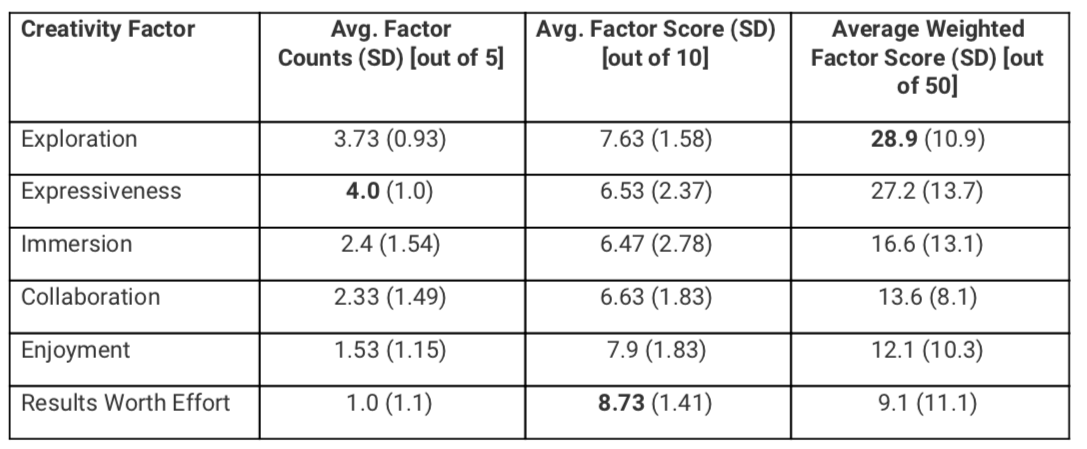
\includegraphics[width=1\textwidth]{pictures/cap4/CSI}
\caption{Resultados do questionário CSI, como os maiores valores médios em negrito.}
\label{fig:questionnaire}
\end{figure}


 
%In another evaluation, PS was tested in controlled lab settings with trios of participants both with and without prior music performance experience. Participants were invited to play three five-minute long free improvisations using the system on their laptops. 15 participants took part in the study (5 females, 10 males, mean$\pm$SD age = 32.7$\pm$5.4), 8 of them considered themselves as musicians (4 intermediate and 4 experienced), while 7 did not. We measured system usability \cite{Jordan1996} and creativity support \cite{Cherry2014} using an online survey to be completed just after the performances. We also conducted inductive thematic analyses \cite{Braun2006} from focus group discussions and self-reports related to workflow, hedonic quality, engagement, learning, contexts of use and improvements. The prototype yielded a high usability score (M = 82.5/100, SD = 8.94) and creativity support index (M =71.7, SD =15.6) with no significant differences between non musicians and musicians.

Nós conduzimos análises temáticas\footnote{\cite{Braun2006}}, tanto doas discussões realizadas após a execução das peças, quanto das respostas e comentários dos usuários apresentados nos questionários. 

Nas discussões realizadas em grupo, reconhecemos os seguintes temas:

\begin{description}
 \item[Satisfação] Sete participantes expressaram verbalmente que gostaram de tocar com outras pessoas usando o sistema

  \item[Expressividade] Três participantes expressaram um grande nível de satisfação sobre a possibilidade de tocar com qualquer tipo de conteúdo sonoro (``Eu gosto do fato de poder pegar imediatamente qualquer tipo de som que vem na minha cabeça e usar isso para compor em tempo real'')

 \item[Monitoramento] Nove participantes mencionaram a impossibilidade de se ouvir o som antes de tocar e desconforto com o fato dos sons serem tocados instantaneamente em volume alto. Alguns mencionaram estratégias para contornar esse problema, eles clicavam bem rapidamente para diminuir o volume do som assim que selecionavam os samples e em seguida faziam manualmente um processo de fade-in.

 \item[Relevância e surpresa] Cinco participantes mencionaram que os sons tocados não correspondiam totalmente as expectativas geradas pelas buscas textuais, que se relaciona com o tagueamento e descrição dos sons no próprio Freesound. Três participantes também mencionaram o fator surpresa como algo interessante para gerar novas ideias sonoras.

 \item[Controle Expressivo] Seis participantes, todos músicos, sentiram necessidade de haver mais controles de expressividade musical, uma vez que naquele momento a interface permitia somente o ajuste de volume de cada som. Eles mencionaram como sugestão um controle geral do volume da página; possibilidade de sincronização das batidas; associação de teclas do teclado com sons; possibilidade de avaliar os sons para ranquear os sons preferidos e a possibilidade de escolher os pontos de início e fim dos loops. Duas pessoas mencionaram que a impossibilidade de sincronização fez com mudassem suas estratégias composicionais (``eu evitei sons com ritmo e procurei sons não musicais'').

  \item[Identificação] Cinco pessoas mencionaram dificuldade em identificar quais sons estavam tocando ou sendo tocados por outras pessoas, um deles sugeriu construir algo colaborativo onde se pudesse ver o que os outros estavam tocando.

\item[Suporte à criatividade e narrativa] quatro participantes mencionaram que tentaram criaruma narrativa em relação ao que os outros estavam tocando, a partir da seleção das palavras-chave em suas buscas (``Eu procurei as palavras-chave para me adaptar ao contexto. Uma ideia de alguém desencadeou outra ideia em mim, então criamos uma narrativa todos juntos'', ``tentei responder ao que os outros estavam tocando, por exemplo, se ouvia ele tocando pássaros, eu procurava encontrar sons de gatos'').

\item[Utilidade dos espectrogramas] Cinco participantes, que tinham fundamentos em tecnologia musical mencionaram que os espectrogramas foram úteis para o processo (``O espectrograma realmente me ajudou a ler os sons e minhas decisões foram baseadas nisso''). Um deles comentou ``é um modo diferente de tocar: eu estou usando meus olhos para tocar música''. Outros cinco participantes, que não conseguiam ler os espectrogramas, relataram que tinham que confiar nas informações fornecidas junto com os arquivos (nome e duração) para tocar.

\end{description}

Nós também fizemos uma análise temática das respostas das questões discursivas apresentadas nos questionários. As 12 questões analisadas foram: 

\begin{itemize}

\item Descreva brevemente seu processo de trabalho usando Playsound

\item O que você mais gostou sobre o Playsound?

\item O que você menos gostou sobre o Playsound?

\item Por favor avalie seu engajamento ao utilizar Playsound para tocar com outras pessoas (Por favor explique brevemente sua escolha)

\item Eu senti que aprendi algo novo ao usar Playsound. (Por favor explique brevemente sua escolha)

\item A forma que compus música usando Playsound foi nova para mim. (Por favor explique brevemente sua escolha)

\item Ao tocar com Playsound que tipos de sons você procurou? (ex. sons musicais, instrumentos acústicos, sons não musicais, gravações de campo, efeitos sonoros, loops, sons de fala)

\item Eu consegui encontrar os sons que eu procurava. (Por favor explique brevemente sua escolha e comente sobre a relevância e qualidade dos sons encontrados)

\item Por favor descreva que melhorias você faria no sistema (ex. interface do usuário, tipos de sons, controles, etc)

\item Por favor descreva em quais contextos de uso você consideraria utilizar o Playsound.

\item Por favor indique algum outro provedor de conteúdo que você estaria interessado em acessar usando uma ferramenta como Playsound

\item Sinta se livre para adicionar qualquer comentário sobre a experiência ou o estudo.

\end{itemize}

A análise temática quantitativa, que foi conduzida por Mathieu Barthet com o auxílio do software MAXQDA\footnote{\url{https://www.maxqda.com/}}, encontrou 681 códigos diferentes nas respostas dos usuários. Os temas mais importantes foram: suporte à criatividade musical (128 ocorrências), busca sonora (64 ocorrências), limitações (61 ocorrências), engajamento emocional (56 ocorrências), técnica de tocar e agência criativa (52 ocorrências), melhorias (44 ocorrências), usabilidade (37 ocorrências) e contextos de uso (24 ocorrências). Abaixo apresentamos um resumo dos resultados encontrados:

\begin{description}
\item[Suporte à criatividade musical e busca sonora] Os usuários relataram frequentemente questões ligadas à criatividade musical, colaboração criativa, expressividade e riqueza dos sons encontrados, como``a possibilidade de tocar qualquer som que viesse à minha cabeça'', ou ``essa ferramenta me permitiu explorar um vocabulário sonoro que eu não costumo usar pra tocar''. Uma grande variedade de conteúdo sonoro foi utilizada durante as sessões, incluindo: sons musicais (ex. relativos a gêneros musicais ou instrumentos); sons temáticos, correspondentes a uma idéia ou tópico; sons de fundo (atmosferas e ambiências); sons de fala (ex. beatbox), efeitos especiais e sons sintéticos (ex. glitches, sons processados espectralmente, sons granulares); sons rítmicos (como padrões e loops de bateria, batidas, etc) e sons relativos à natureza (ex. ``pássaros'').

\item[Limitações] As limitações apresentadas pelos usuários sobre o sistema incluíam questões relacionadas à barreiras criativas e questões técnicas. Quanto às barreiras criativas, houveram menções ao fato de não ser possível reconhecer o que estava sendo tocado, sobre a curva de aprendizado, aleatoriedade dos resultados, falta de controle, falta de feedback sobre as atitudes dos outros. As questões técnicas foram relativas à falta de controle, falta de monitoramento, para saber o que seria tocado de antemão, controle do volume, relevância dos sons, metadados e qualidade sonora (ex. variação de dinâmica e equalização de volume)

\item[Engajamento emocional e estratégias de tocar] Um grande número de ocorrências (56) mencionam um engajamento emocional positivo com o sistema e as tarefas. Frequentemente mencionaram satisfação (18), engajamento (15), diversão (8), interesse (6), fluxo (5) e imersão (3). Muitas ocorrências (52) descrevem uma série de técnicas ou estratégias empregadas pelos participantes. Elas incluem tocar por idéias semânticas, liderar a composição, tocar ritmicamente, usar loops, tentar procurar sons semelhantes, tocar através de ideias musicais, sobreposição de camadas de sons, ser inspirado pelos outros, usar descoberta generativa, adicionar elementos faltantes ou divertidos, tocar randomicamente, por tentativa e erro, etc. Essa lista longa de estratégias possíveis foi um bom indicativo de que o sistema era útil como suporte para criatividade musical. 

\item[Melhorias] O participantes indicaram várias melhorias possíveis para o sistema (44 ocorrências). Muitos aspectos relativos aos processos de controle sonoro, como melhor controle do volume e do loop, velocidade do sample, efeitos especiais, filtros e interface para controladores externos. Muitos mencionaram a falta de um monitor para ouvir os sons em um fone de ouvido antes de tocar, recurso que exigiria o uso de uma interface de áudio externa. Sugeriram também processos para sincronizar, ou agrupar sons, busca por parâmetros sonoros, como BPM ou gênero, por exemplo. Outro ponto comentado foi quanto a percepção do que se está tocando e do que os outros estavam tocando. Também foram mencionados aspectos de controle de dinâmica como fades automáticos, controle geral de volume e compressão de áudio. Outras fontes de conteúdo sonoro possíveis mencionadas foram Youtube e RedPanal.

\item[Usabilidade] Aspectos de usabilidade foram notados. A simplicidade do sistema e clareza da interface foi notada por alguns participantes. Um deles apontou que ``é muito intuitivo''. Quanto ao uso dos espectrogramas, houveram menções em sentidos opostos. Alguns acharam útil enquanto outros não, fato que está relacionado com a experiência dos usuários nesse tipo de representação. Alguns usuários solicitaram mais informações para auxiliar a escolha dos sons. Muitos apontaram também positivamente a velocidade do sistema eu facilidade para encontrar os sons.

\item[Contextos de uso] Vários contextos possíveis de uso foram apresentados pelos participantes, como: improvisação livre; pesquisa de sons e samples; trilha sonora para vídeos; improvisações de dança; orquestras de laptop; como ferramenta de rascunho para produções musicais posteriores; composição de paisagens sonoras ou para se divertir.

Apesar de consumir um grande esforço, a realização dos testes com usuários foi uma experiência muito produtiva para o desenvolvimento do sistema. A possibilidade de obter feedback de pessoas de fora do projeto, e de testar como o sistema poderia ser utilizado por outras pessoas foi muito rica e os comentários observados foram bastante significativos. Para os usuários com mais experiência em música, a simplicidade e a não constrição a uma estrutura de grade rítmica foi notada com certo desconforto, enquanto os usuários sem experiência prática musical puderam usar o sistema com mais facilidade, todo, no entanto, foram capazes de tocar em conjunto e produziram resultados musicais interessantes. Isso foi de encontro à proposta inicial do projeto de criar uma ferramenta intuitiva direcionada a pessoas sem domínio de técnicas musicais, e gerou ideias para o desenvolvimento do projeto. O material gravado durante as sessões também serviu para produzir um pequeno vídeo demonstrativo do sistema \footnote{Disponível em: \url{https://youtu.be/yv8T70rawzs}}, que foi apresentado na reunião do projeto Audio Commons em Luxembrugo no mês de fevereiro de 2018. 



\subsubsection{Avaliação prática}

Pouco tempo após a realização dessa avaliação mais formal em laboratório, tive a oportunidade de testar o sistema na prática em uma performance solo, no evento A'mas que aconteceu no Total Refreshment Centre em Londres, no dia 25 de Março de 2018\footnote{Um trecho da performance pode ser assistido em: \url{https://youtu.be/LmjmpQagBG8}}. Para a ocasião, decidi trabalhar com um material pré-selecionado, para garantir uma consistência durante a performance. Depois de uma performance solo de 30 minutos, onde toquei com o sistema e pratiquei improvisação vocal. Decidi por fazer uma seleção de bases, que usei para criar texturas e variações de ritmos durante a performance. 

No final, também participei de uma jam session com os outros 8 músicos. durante a jam, uma parte dos músicos estava conectada através de um relógio MIDI central, que sincronizava o BPM dos sistemas baseados em grid, como Playsound não é baseado em grid, tive que desenvolver estratégias específicas para não entrar em conflito com a grade musical que se estabeleceu. Isso incluiu tocar com texturas mais longas e não rítmicas, tocar com o botão play no ritmo (dispensando o recurso de loop), saturar elementos curtos em alguns momentos.

Apesar de ter sido possível tocar, houveram alguns problemas que notei durante a performance. Quando empregamos sons pré-selecionados, tivemos alguns problemas relativos a performance do computador devido a um sobrecarregamento da mémória. Além disso, senti o grau de controle de processos sonoros poderia ser desenvolvido para melhor aproveitamento dos materiais sonoros durante a performance.

\begin{figure}

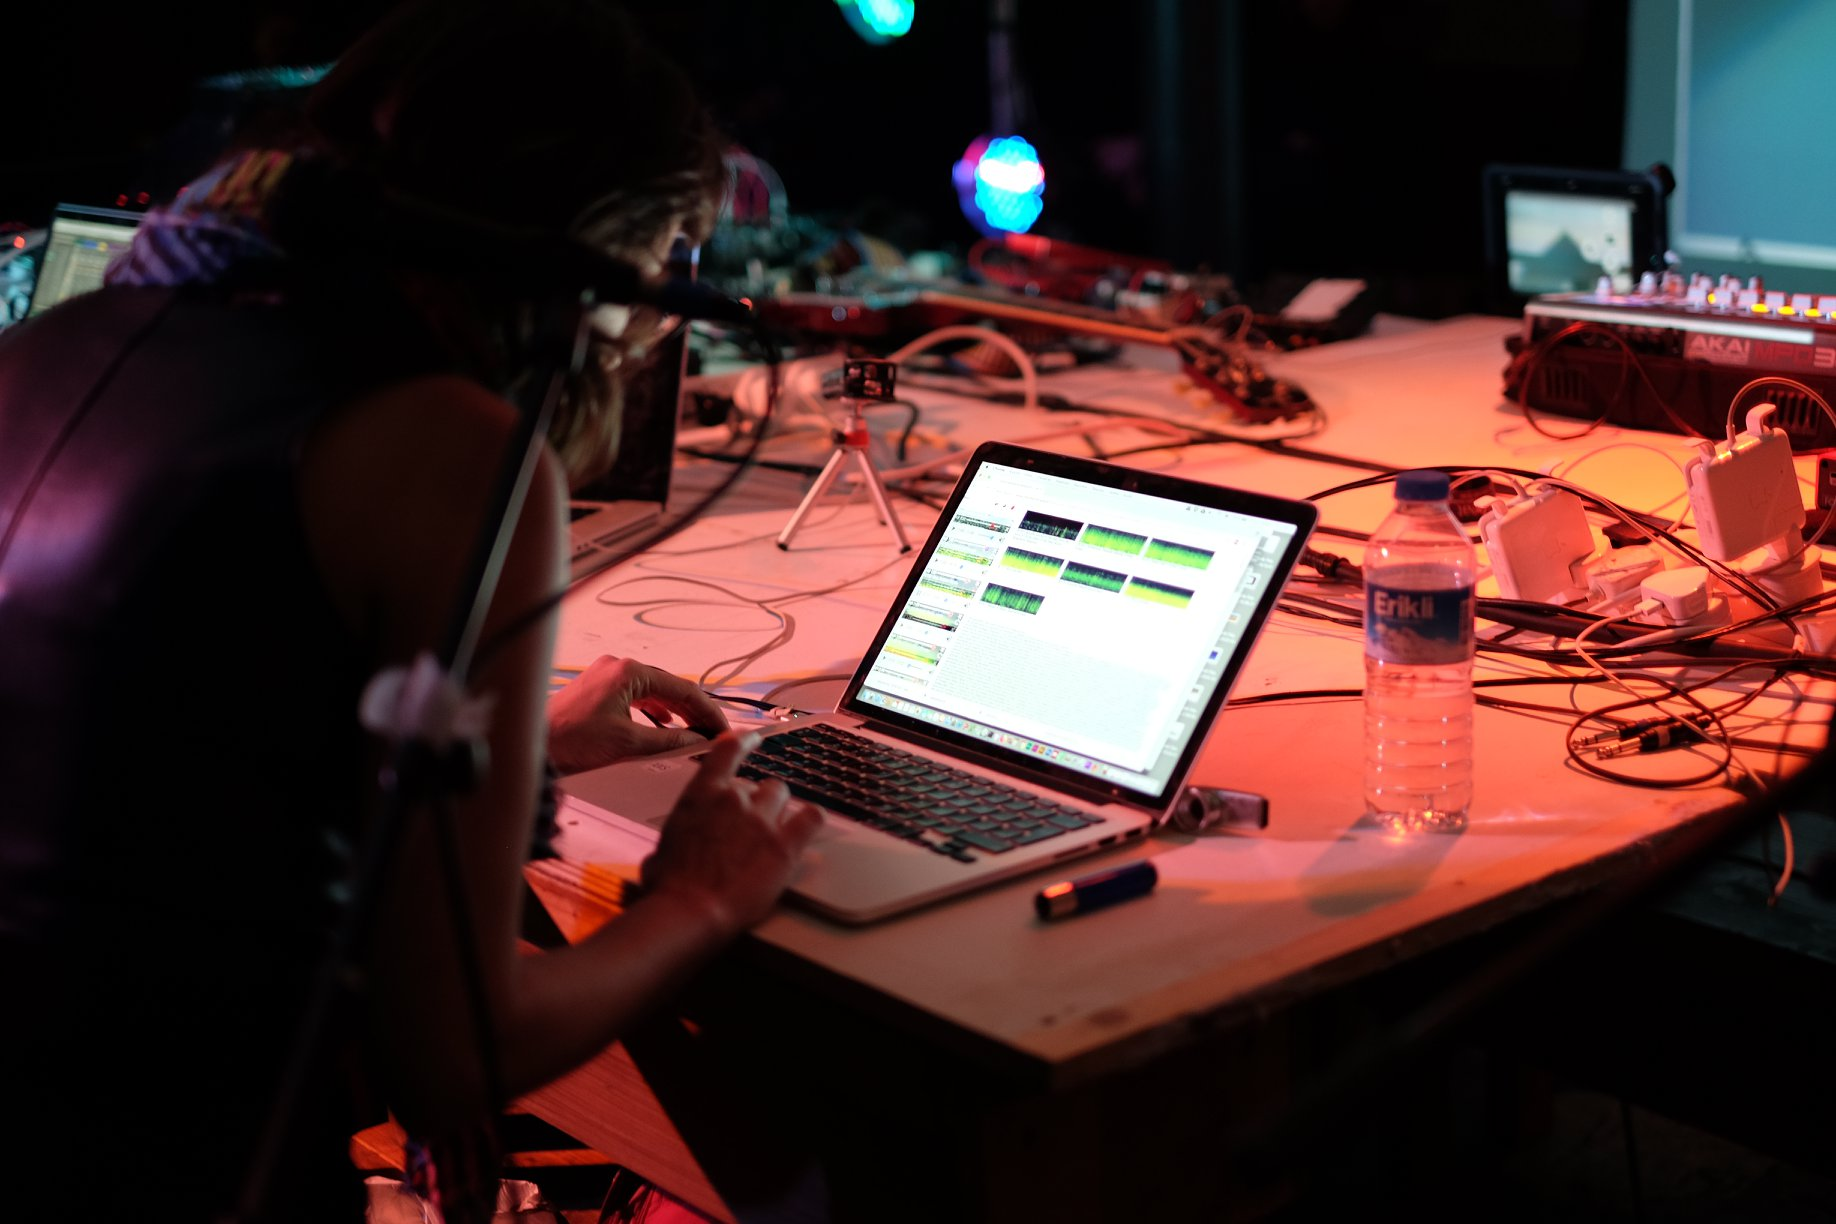
\includegraphics[width=1\textwidth]{pictures/cap4/ariane_amas}
\caption{\label{amas}Performance solo no evento A'mas em Londres.}
\label{fig:amas}
\end{figure}


\end{description}





%These initial user evaluations were followed by a first live solo performance with PS by the first author at the A'mas event held at the Total Refreshment Centre in London on 25 March 2017 \footnote{Excerpt from the performance can be found at \url{https://youtu.be/LmjmpQagBG8}}. After a 30 minutes solo performance, the performer also joined a jam session with 8 other invited musicians who played synthesizers and other electronic instruments. During the jam, most of the instruments were connected through a central Midi clock providing beat synchronization. Although PS does not offer this possibility, since it is not grid-based, it was still possible to play live in this format. The performer had to develop a strategy to select in real time sounds that wouldn't conflict with the established rhythm, working with sonic materials such as textures and effects instead of more structured loops. By using this system as part of a public live electronic performance, we acknowledged that it could be used as a basis for real music practice. But as in previous evaluations, the performer also found that the creative control would benefit from enriched audio processing.



%``Non musician, Sophie''
%I got more and more into it the longer I played around with it and I think that the longer we all played together, the more coherent outcomes we produced. despite the difficulties of not always knowing to what extend I contributed what sounds, it was still enjoyable to listen to the atmosphere we managed to create.


%I tried to listen to other musicians and react to their playing. Some times I instead took the initiative to propose my ideas, even if they were not coherent with the narrative proposed by the others. This was to create something new, to give another direction to the music


\subsection{Playsound WebAudio}

Em seguida a esse primeiro círculo de desenvolvimento e avaliações, meu desejo era o de trabalhar no desensenvolvimento do tocador de áudio. Naquele momento, estava trabalhando como professora auxiliar no curso de ``Creative Coding'' (programação criativa), que estava sendo ministrado por Alessia Milo na Universidade de Greenwich. O curso abordava tópicos como o uso de tecnologias web e API's em projetos artísticos, afins a
 esta pesquisa. Ela se interessou em colaborar com o desenvolvimento do projeto e implementar tecnologias que permitissem um maior controle e processamento dos sons tocados.

 A partir das análises das experiências realizadas, organizamos uma lista de demandas prioritárias para trabalhar, também observamos que algumas demandas apontadas pelos usuários, por exemplo, iam de encontro com necessidades que também senti como performer, enquanto outras eram divergentes dos objetivos gerais do projeto.

 A questão da sincronização de batidas, por exemplo, que alguns usuários mencionaram (todos eles músicos experientes), não é prioritária, uma vez que já existem várias opções de software profissionais para atender essas demandas, e um dos princípios norteadores desse trabalho era de propor algo que pudesse ser tocado sem esse tipo de constrição. Outro ponto apontado por alguns usuários seria a criação de um sistema para monitoramento dos samples antes de tocar. Para que isso seja possível, é necessário o uso de uma interface de áudio externa, o que diminui também a acessibilidade do site. Gostaríamos de manter o foco da pesquisa justamente em desenvolver soluções que não exijam a instalação de nenhum outro equipamento para tocar, além do computador ou celular com acesso à internet. 

 Uma questão que abordamos foi o fato dos sons sempre tocarem instantaneamente com a seleção, em volume médio. Alguns voluntários apontaram essa questão, que também senti na prática durante a performance solo. Para contornar essa questão, mudamos a forma com que os sons são tocados. Na nova versão, ao clicar na imagem correspondente ao som, o som é colocado na playlist, mas ele não toca, então é possível selecionar o volume desejado antes de tocar o sample. Adicionamos também um pequeno botãozinho de play sobre a imagem, que permite ainda tocar instantaneamente o som desejado.

 Desenvolvemos também a interface, para que fosse possível selecionar um trecho do loop para tocar. Para implementar esse recurso, mudamos toda a base do processamento de áudio do sistema. Enquanto a primeira versão se apoiava nos elementos HTML para tocar, na nova versão passamos a empregar a WebAudio API de forma mais direta, através do elemento \emph{buffer}, que carrega os sons na página e os manipula diretamente através de JavaScript. Implementamos também \emph{panning}, para distribuir os sons nos canais estéreo, e o controle da velocidade de reprodução do sample (\emph{playbackrate}), que permite mudar também o tom do sample (alterando também a duração em conjunto. Nas figuras \ref{handbell} e \ref{handbelldt}, que apresentam espectrogramas da peça da autora``Handbell'' \footnote{Disponível em: \url{https://soundcloud.com/asss/handbell}}, feita a partir da manipulação de um sample usando PS, podemos notar as capacidades transformativas dos novos recursos adicionados. 



\begin{figure}

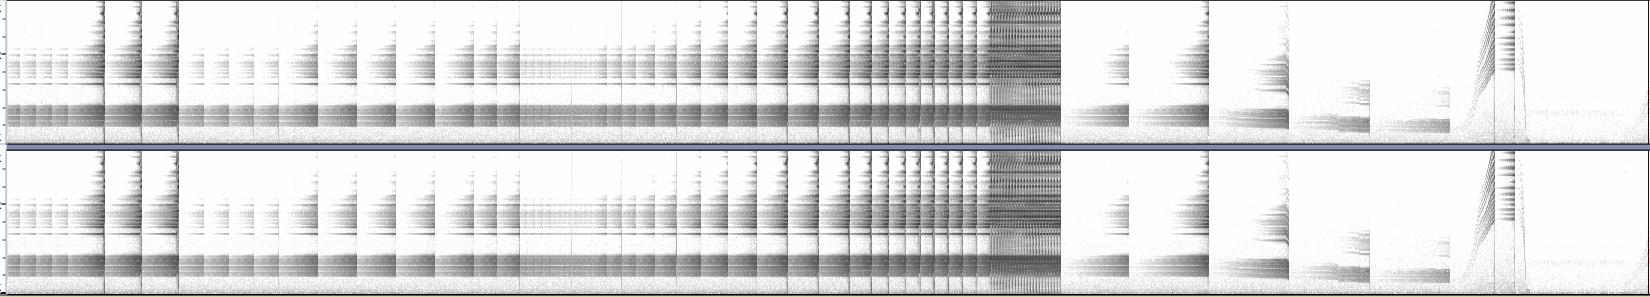
\includegraphics[width=1\textwidth]{pictures/cap4/handbellreverse}
\caption{\label{handbell}Espectrograma da peça Handbellreverse.}
\label{fig:handbell}
\end{figure}




%\subsection{Melhorias}

%Following users' desire for more expressive control, we added a range of audio editing, processing and mixing capabilities. This included the possibility of queuing sounds in the playlist and manipulating their duration and pitch by varying their playback speed. We also enabled editing by selecting segments and control custom loops during playback. To implement this feature, we used the buffer object from the Web Audio API library which replaced the HTML media element object (despite the HTML media object can start playing upon selection large files while still buffering). We also introduced a panning control for each sound object, allowing to position them in the stereo field. We are planning to introduce a panning control on the master channel e.g. to help musicians from laptop ensembles to identify individual sonic contributions spatially.



\begin{figure}

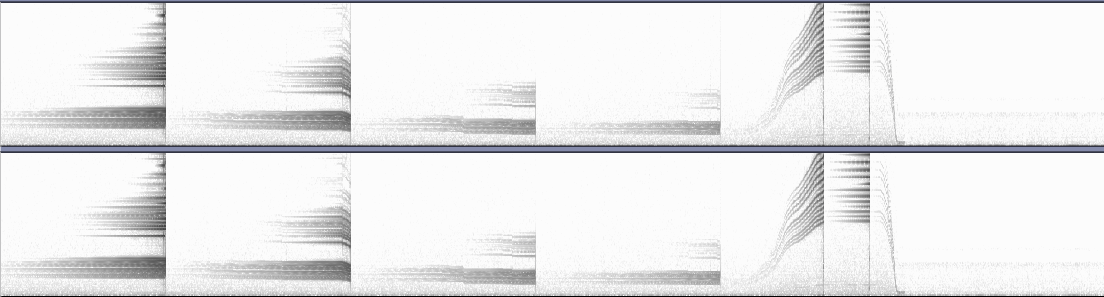
\includegraphics[width=1\textwidth]{pictures/cap4/handbellreverse_detail}
\caption{\label{handbelldt}Detalhe do espectrograma da peça.}
\label{fig:handbelldt}
\end{figure}


Uma mudança importante da primeira versnao para a segunda, que na verdade não é uma melhoria mas uma restriçnao, foi motivada por discussões éticas quanto à questão dos direitos autorais e licensas dos sons. Enquanto na primeira versão oferecíamos acesso a todos os sons do banco de dados do Freesound, independente da licensa. Decidimos restringir o acesso somente aos sons com licensas Creative Commons 0 (que equivale ao domínio público) e Attribtion, que exige a citação do autor dos sons originais. Essa decisão, que excluiu uma quantidade relativamente pequena de sons\footnote{Em um levantamento em novembro de 2018, haviam 395183 sons no total no banco de dados do Freesound, sendo que deles 47361 tinham licensa atribuição não comercial.}, mas muitos deles de boa qualidade foi motivada não só por uma questão de evitar possíveis problemas legais decorridos do uso do software, como também por uma questão ética, de incentivar o uso de licensas livres por parte dos usuários do Playsound. Dessa forma, se um músico quiser utilizar seus próprios sons na plataforma\footnote{Como fizemos por exemplo na performance Tender Buttons | Sound | Space, que está descrita mais adiante nesta tese}, deverá necessariamente publicá-los com uma licensa menos restritiva. 

Em conjunto com a implementação deste filtro, colocamos também na interface do site uma seção de créditos, que se atualiza automaticamente na medida em que sons com a licensa de ``Atribuição'' são tocados. Desta forma é fácil para alguém que queira fazer uso dos sons gerados pela ferramenta de dar os devidos créditos aos produtores de conteúdo original. 

Na segunda versão, colocamos também em cada player, um link para a postagem do som original no Freesound, para quem quiser baixar o áudio em alta qualidade para fazer uso em algum outro programa de edição, por exemplo. 



\subsubsection{Teste com a Orquestra Errante}
Os testes com usuários feitos em laboratório foram úteis para comparar o sistema com outros projetos que também estavam sendo desenvolvidos no contexto do projeto Audio Commons, mas apesar disso, estávamos mais interessados em avaliar como o instrumento se sairia em condições mais realistas de uso. Para isso, seria interessante testar o projeto com grupos musicais já estabelecidos. Ao término do meu estágio de pesquisa na QMUL e antes de assumir a vaga de professora na Universidade Federal do Sul da Bahia, tive a oportunidade de passar alguns dias em São Paulo, onde consegui marcar uma sessão de avaliação do PS com a Orquestra Errante, grupo coordenado pelo professor Rogério Costa, do qual também faço parte. Avaliando criticamente o processo de avaliação em laboratório na QMUL, decidi concentrar os esforços na avaliação prática do instrumento, e otimizar o tempo dos músicos no ensaio, deixando o preenchimento do questionário como opcional para quem quisesse responder fora do horário do ensaio. No final, apenas 3 dos oito participantes preencheram o questionário, o que inviabilizou as análises quantitativas

A dinâmica do trabalho do grupo é não hierarquizada, onde ``a criação se dá sempre de forma colaborativa, coletiva, compartilhada em tempo real e irrepetível.'' \footnote{\cite{costa2013orquestra}}. O grupo sempre discute as propostas musicais apresentadas e como elas devem ser executadas pelo coletivo dos músicos. Sendo assim, deixamos também para discutir com os músicos no dia do ensaio os procedimentos que seriam seguidos e os arranjos para organizar os grupos para testar o sistema para a prática de improvisação livre. Nós decidimos conjuntamente organizar o grupo para tocar três peças curtas (de cerca de 2 minutos) em trios, com um usuário do sistema e dois músicos tocando seus instrumentos tradicionais e três peças mais longas (de tempo livre) com dois músicos tocando PS e os demais tocando seus instrumentos conjuntamente (Figura \ref{psorquestra}). Em cada sessão foram alternados os usuários do sistema de modo que todos membros da Orquestra puderam experimentar com a ferramenta. Antes de tocar, os músicos tinha um período curto de familiarização com o instrumento que levou cerca de 3 a 8 minutos, dependendo do músico. Depois de cada sessão, discutimos coletivamente sobre o instrumento e a sonoridade resultante de seu emprego no processo de improvisação.


Participaram do ensaio os músicos: Miguel D. Antar (contrabaixo acústico), Marina Mapurunga (violino com efeitos), Fábio Martinez (saxofone e piano), Fábio Manzone (percussão), Rogério Costa (saxofone), Caio Rigui (flauta) e Stênio Biazoni, e Yonara Dantas, que não se considera musicista, mas participou também do ensaio tocando a ferramenta. A tabela \ref{tab:orchestra} mostra a formação e a duração de cada uma das sessões tocadas\footnote{A sessões foram gravadas e o registro pode ser escutado em: \url{http://finetanks.com/records/playsound/orquestraerrante}}.  

\begin{table}[ht]
\caption{Configuração de instrumentos e duração das peças durante o ensaio com a Orquestra Errante.}
\begin{tabular}{ll}
\textbf{Instrumentos}                                                    & \textbf{Duração} \\
PS + contrabaixo + violino                                & 2:34"         \\
PS + percussão + voz                                                 & 3:40"         \\
PS + flauta + sax                                                        & 2:30"         \\
PS + PS + percussão + voz + sax + flauta + piano                      & 8:04"         \\
PS + PS + sax + voz + contrabaixo + flauta + piano                   & 7:03"         \\
PS + PS + percussão + voz + contrabaixo + violino + flauta + sax & 14:51"       
\end{tabular}
\label{tab:orchestra}
\end{table}



\begin{figure}

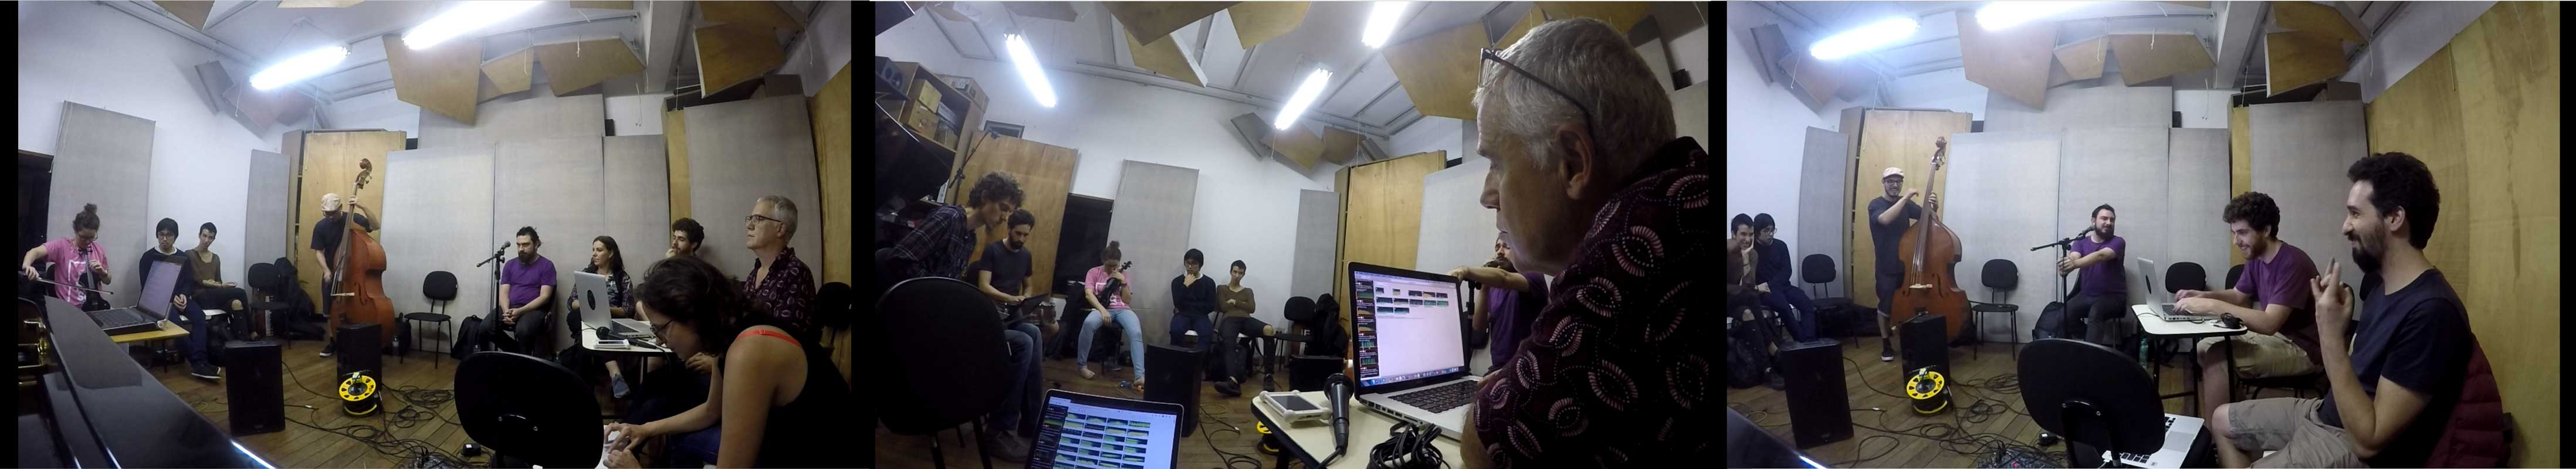
\includegraphics[width=1\textwidth]{pictures/cap4/orquestra_errante_usertest}
\caption{\label{psorquestra}Avaliação com a Orquestra Errante.}
\label{fig:psorquestra}
\end{figure}

\subsubsection{Análise das performances}

Ouvindo as gravações do ensaio, percebemos que comparando com o teste anterior, os membros da Orquestra preferiram trabalhar com menos materiais sonoros e passar mais tempo explorando o processamento do som, ao invés de buscando sons novos. Isto pode ser devido à implantação de novos recursos para processamento de áudio, que permitem trabalhar desdobramentos musicais de um mesmo som com mais ricos do que na versão anterior, onde só havia controle de loop e volume, mas também pode ser relacionado com a experiência dos músicos em improvisação musical, que os levou a trabalhar mais no campo da sonoridade e exploração desses aspectos mais sutis de variação sonora. As peças apresentadas possuem um grau elevado de variação de dinâmica e texturas, dependendo da configuração dos grupos. Houveram interessantes diálogos musicais entre os musicistas, com diversas situações do tipo ``pergunta e resposta'' e diferentes relações de figura e fundo entre o PS e os instrumentos tradicionais. Algumas vezes, os músicos tocando PS produziram texturas onde outros músicos puderam improvisar em conjunto, em outras, agiram como solistas se destacando do contexto geral, como é de praxe nos ensaios regulares e apresentações públicas da Orquestra. 



%Audition of the recordings showed that, comparing to the previous tests, most performers from the improvisation ensemble chose to work with fewer sonic materials and spend more time at exploring sound processing instead of using large amount of sound samples. This may be due to the richer amount of expressive controls present in the updated interface, but also a will to closely work with sonorities, which is characteristic of FMI. The performed pieces present a great degree of variation in dynamics and textures, depending on the group configurations. There were interesting musical dialogues between the performers, with question-response situations and different ground-figure relations between PS and traditional instruments. At times, PS players produced accompanying textures and in other occasions, they acted as soloists, as commonly takes place in the practice of the ensemble.


\subsubsection{Análise temática}
Para conduzir a análise temática\cite{Braun2006}, transcrevi os diálogos das discussões com o grupo e as três respostas dadas nas questões discursivas, que foram versões traduzidas das mesmas aplicadas nos testes na QMUL. Nós identificamos em uma tabela em Excel, os temas seguintes, que também estavam presentes na análise da versão anterior do projeto\footnote{\cite{Stolfi2018b}}.

%We conducted a thematic analysis \cite{Braun2006} on the transcriptions of the group discussion and answers to the survey. We identified the recurrent themes below which were also present in the previous analysis \cite{Stolfi2018b}.

\textbf{Suporte à criatividade e narrativa.} (10 ocorrências) Usuários comentaram sobre o processo de tocar juntos (\textit{``o som que você tocou influenciou diretamente o que eu ia fazer, o contrário também aconteceu''}, \textit{``sim, eu mudei a velocidade em função do que você tocou"}), and sobre o tipo de sons tocados (\textit{``alguns sons interessantes fora de contexto que nós abraçamos, mas que foi quase no limiar do riso"} ). 

\textbf{Relevância e surpresa.} (7 ocorrências) Alguns participantes demonstraram excitação ao tocarem com a ferramenta (\textit{``a gente pode brincar?"}, , \textit{tem todos os sons do universo} \textit{``sonoramente está bem resolvido"}).

\textbf{Engajamento emocional e estratégias para tocar} (10 ocorrências) Participantes relataram a novidade da ferramenta que permitia uma forma diferente de tocar (\textit{``isso gera uma forma de tocar específica"}, \textit{``são amostras interessantes que você pode manipular como um objeto sonoro"}, \textit{``a sacada é a busca por palavras"}), e sobre como eles usaram a ferramenta durante as performances (\textit{``eu fiquei tocando, depois eu mudei o tempo, e depois usei pra selecionar os trechos de loop"}).

\textbf{Limitations.} (9 ocorrências) Os usuários relataram questões relativas à interface no momento, que deixava confusa a qual áudio os controles se relacionavam, e sobre a falta de feedback visual de qual arquivo estava tocando. Durante o estudo, a interface apresentava um \emph{bug} no elemento que indicava a posição de cada sample tocado. Os participantes também reclamaram da velocidade de resposta, uma vez que a internet estava bem lenta no estúdio e a versão atual, que funciona através de buffers, exige que se descarregue todo arquivo antes que se possa tocá-lo.


%Users reported some issues with the current interface, that had misleading controllers and lack of visual feedback about the sounds being played. During the study, the interface faced a bug preventing the playhead positions to show the current position in each audio sample. Participants also commented on the speed of the response, since the Internet speed was very slow during the test.

\textbf{Identificação de sons e fontes sonoras.} (3 ocorrências)  Usuários reportaram que foram capazes de identificar os sons digitais. Um dos participantes relatou dificuldade em reconhecer que estava tocando o quê e outro sugeriu que a performance seria melhor se cada participante tivesse seu próprio conjunto de caixas de som.

\textbf{Melhorias.} (12 ocorrências) Os participantes sugeriram melhorias desejáveis como: incluir a possibilidade de mudar a duração do som (sem alterar o pitch), sincronização de todos os sons, controle para parar todos os sons ao mesmo tempo, incluir suporte para controladores MIDI, opções de fade-in e fade-out para cada som, e interface com outros tipos de hardware, como Arduino e Raspberry Pi. 

Na resposta do questionário sobre o que os participantes mais gostaram a respeito do PS, eles mencionaram a quantidade de sons disponíveis e empoderamento (\textit{``senti uma espécie de poder por ter disponível uma imensa quantidade de sons para usar"}), e sobre a possibilidade de combinação de sons \textit{``As texturas com várias camadas sobrepostas''}. Sobre o tipo de sons pesquisados, os usuários reportaram a busca por  \textit{``sons não musicais"} e \textit{``sons graves, da natureza"}, curiosamente, um terceiro afirmou: \textit{``não procurei nada. Os sons vieram de encontro a mim."}.

\subsubsection{Chat}
Um desejo que esteve presente desde as primeiras ideias para esse software era de desenvolver uma plataforma colaborativa para performances coletivas. Quando fizemos a primeira avaliação, no laboratório da QMUL, os participantes da experiência também relataram desejos de se estabelecerem formas de comunicação entre os participantes.

Começamos então a desenvolver uma interface para um sistema de chat cujo protótipo já está em funcionamento. Entrando no endereço \url{http://www.playsound.space/chat} o usuário é direcionado para uma sala de bate papo onde por enquanto é possível se compartilhar somente texto\footnote{Em uma próxima versão do projeto, pretendemos que seja possível compartilhar também o som gerado por todos participantes}. Cada palavra na janela do chat também se torna um link conectado ao campo de busca. Com isso é possível compartilhar informação entre os usuários conectados ao sistema.

Na versão atual, o chat é baseado na tecnologia de comunicação via websockets, que foi implementada na versão atual em node.js através do uso da API socket.io. Atualmente, estamos em processo de desenvolvimento de uma nova versão do software, que permitirá aos usuários a criação de salas individuais de bate papo e compartilhamento dos processos sonoros.
%The chat is based on socket communication, implemented in node.js through socket.io. Ids are assigned automatically to the clients accessing the address, and we are currently implementing the creation of user-defined chatrooms.





%Since the last evaluation, we have included new features which will be the object of future evaluations. These features have been developed mostly to enhance participatory processes, by providing a chat environment, and accessibility, through a built-in translation system aiming to let non-English speakers use the tool.

%At the address \url{http://www.playsound.space/chat}, the user can type messages that are shared with other users connected to the same address. Moreover, the messages, once sent, become hyperlinks which, when selected, trigger a query in the Freesound database. This in return shows results for the related word. 


\subsection{Tradução}

Outra questão, que ficou ainda mais clara quando voltei ao Brasil foi de que o idioma seria uma barreira significativa para a acessibilidade do sistema. A busca na API do Freesound, é feita por um mecanismo que simples que funciona através de buscas textuais no banco de dados do site, que é construído majoritariamente em inglês. Para falantes de outra línguas, o acesso ao conteúdo do site passa por essa barreira da linguagem. Como tínhamos como objetivo desenvolver um sistema que também pudesse ser utilizado em aulas e oficinas para o estudantes no Brasil, o que nos motivou a implementar um sistema de tradução interno, que por enquanto só funciona dentro do chat, que nos permite selecionar a língua de entrada e a língua de saída, incluindo inglês, que é a língua principal nos metadados do Freesound. Esse sistema foi implementado pelo engenheiro de computação Fábio Viola, que colaborou durante alguns meses como pesquisador pos-doc no projeto Audio Commons na QMUL. Ele também começou a desenvolver um sistema de recomendações semânticas\footnote{\cite{Viola2018}}, que sugeria conteúdos relacionados de outros provedores como Jamendo e Europeana. Infelizmente, o desenvolvimento foi interrompido antes que fosse possível chegar em um protótipo funcional que pudesse ser empregado em performances ao vivo.

O sistema de tradução implementado é baseado na API Yandex\footnote{\url{https://tech.yandex.com/translate/}}, que suporta 90 línguas diferentes. No entanto, para facilitar a seleção, reduzimos a possibilidade às 17 línguas mais presentes no banco de dados do Freesound. Quando se digita uma palavra no campo de busca, a API sugere uma tradução, que pode ser selecionada pelo usuário para uma nova busca na língua desejada.

Para exemplificar a utilidade da ferramenta de tradução, podemos testar um exemplo, baseado na palavra em português ``pandeiro'' (``tambourine'' em inglês). No momento que implementamos a ferramenta, o Freesound tinha como resultado, 52 sons que continham a palavra no nome, descrição ou tags, se traduzirmos para o inglês, conseguimos 460 resultados com a mesma busca. mar = 274 sea = 2471
serra = 394
saw = 3662

%Freesound APIs \footnote{https://www.freesound.org/docs/api/overview.html} propose a text search mechanism that operates by matching tags and other metadata. This simple mechanism (exploited by PS) does not account for mismatches between the language that users employ in their queries and the ones used in tagged Freesound content. As this can impair the inclusion of non-english speakers, it motivated us to implement a translation tool, which now allows the user to select its own language and receive possible translations to English, the main language of the metadata. 

%Playsound's translation tool relies on Yandex APIs\footnote{\url{https://tech.yandex.com/translate/}}, that supports 90 languages. To simplify the interface, we reduced the range to 17 languages that are more present on Freesound. When users type in a keyword in the research field, PS issues a request to the translate API and propose the results to the users. They are then allowed to click on the suggestion to start the research with the English keyword.

%To illustrate how the translation tool can be useful for a user we provide an example based on the Portuguese word \textit{``pandeiro"} (i.e. tambourine in English). At the time of writing, Freesound hosts 52 sounds matching the word ``pandeiro". If Portuguese is set as the input language, PS translation let users query sounds with the English translation of the word, which yields 460 results.

%\subsection{Tag and Audio Content-based Recommendation}

%Another feature which we develop in parallel provides recommendations of audio files that sound similar to selected ones\footnote{\cite{Viola2018}}. This contribution is framed within the EU-funded Audio Commons project that aims at easing the access to Creative Commons audio content to the creative industries. The implemented recommendation mechanism is a complex multi-agent system based on the Semantic Web of Things. It operates through a two-stages approach: in the first stage it looks for audio files with the same tags on Freesound as well as on Europeana and Jamendo (all these three are content providers of the Audio Commons Ecosystem). In the second stage, an audio analysis is performed to reject results that differ too much from the originally selected file (at the moment a simple similarity function is implemented using spectral linear centroid computed with Sonic Annotator and Vamp plugins\footnote{\cite{Cannam2010}}).

%\section{Discussion}

%There are currently three instances of Playsound that are developed in parallel. The main instance can be used as a single user instrument or composition tool. The version including the chat system will be developed to become a fully participatory music making tool. The Playsound recommendation system should include in the future sounds from other resources and be integrated into the other instances upon positive result from testing. While some of the features developed came from necessities identified among the test users, other features followed design choices discussed by the authors to better support inclusion (for example the translation system) and to provide access to the Audio Commons Ecosystem (recommendations). Even though tests were made with different users during different phases of development, the core of the analysis mostly comes from the author's continuous practice with the system itself. Eventually, we realized that although porting the system to Web Audio buffers may offer more support in music processing, it also makes the system loose part of its real-time playing capabilities, as currently sound buffers need to be fully loaded before playing.



\subsection{Aplicação Prática}
Após essas primeiras rodadas de avaliação, tive a oportunidade de aplicar o uso do instrumento em uma série de atividades práticas, como aulas, concertos e performances. 


\subsubsection{Curso de Edição, Captação e Produção de Audio Digital}

Voltando ao Brasil, assumi a vaga de professora efetiva na UFSB, para ministrar principalmente cursos para a habilitação em ``Arte e Produção Sonora'' do curso ``Som e Imagem em Movimento''. No primeiro componente que ministrei ``Edição, Captação e Produção de Áudio Digital'', que ministrei em conjunto com o professor Leonardo Souza, do curso de artes do corpo em cena.

Pudemos usar a ferramenta em diferentes contextos educacionais. Numa aula sobre timbre, por exemplo, reunimos num link vários exemplos de uma mesma nota gerada por instrumentos diferentes como diapasão, violino, clarinete, oboé, trompete, flauta, voz, piano, guitarra elétrica e diversos modelos diferentes de sintetizadores facilmente a partir do acervo do Freesound. Pudemos tocar todos esses sons facilmente e compará-los inclusive analisando e explicando os diferentes perfis de espectro de frequências sonoras.

Numa segunda oportunidade, o professor Leonardo trouxe uma série de playlists com diferentes tipos de sons como glissandos, batidas para realizar uma atividade de preparação de corpo sonoro com a turma de alunos. Um dos alunos operou com facilidade essas playlist improvisando com os sons reunidos enquanto o professor coordenava a atividade de corpo. 

Mais adiante no curso, quando partimos para produção musical, passamos a utilizar outras ferramentas como editores de áudio e trackers com sintetizadores e samplers. Nesta fase, usamos o Playsound principalmente para pesquisar sons para serem adicionados aos projetos dos alunos, que foram montados posteriormentes nos sequenciadores. Essa breve experiência foi importante para testar vários potenciais de aplicação do Playsound também na esfera educacional. Por ser livre, aberto e sem a necessidade de instalação, é uma ferramenta versátil que pode ser adotada por educadores em diversas práticas.

\begin{figure}

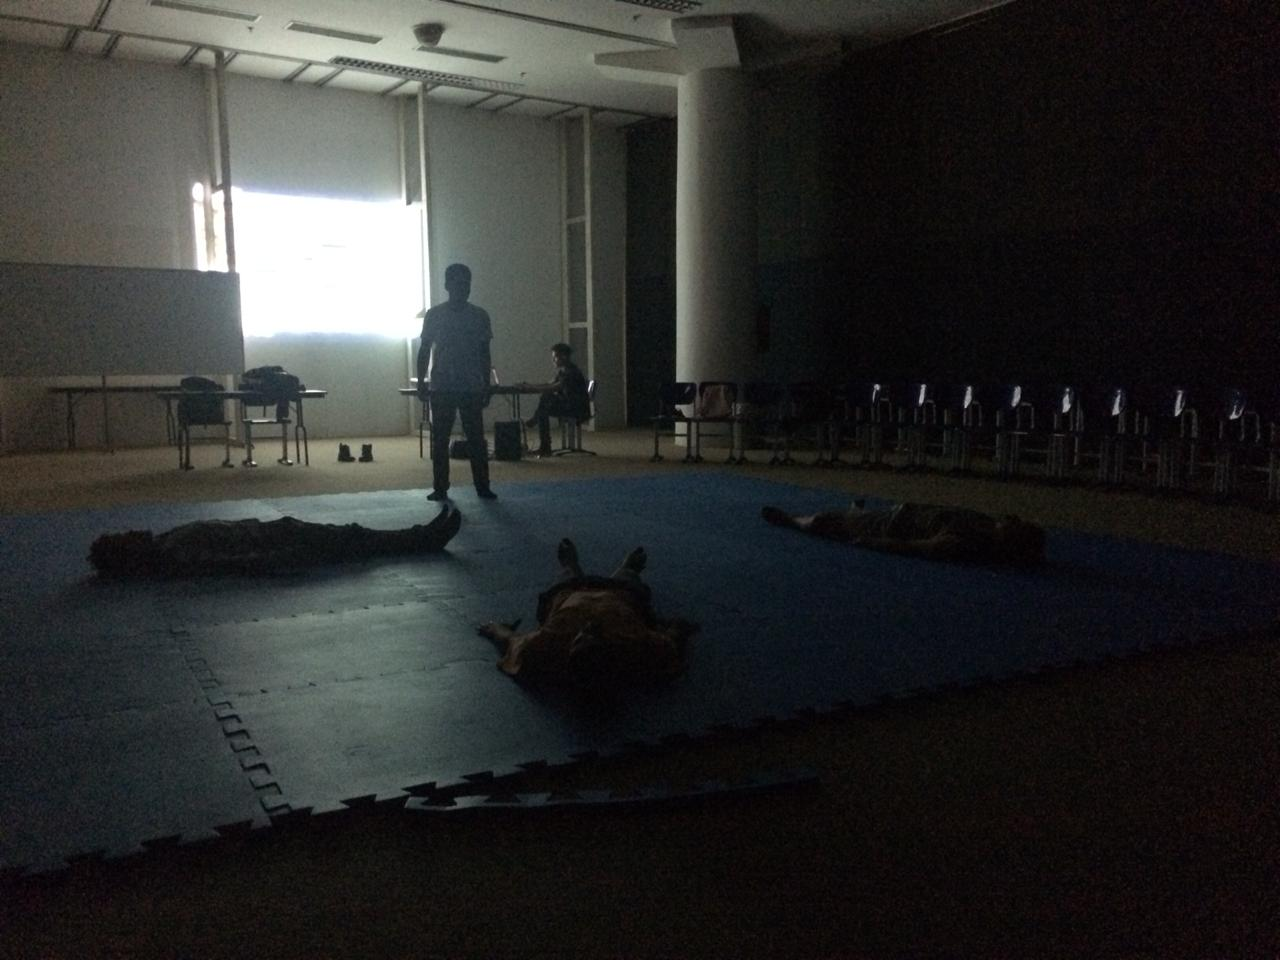
\includegraphics[width=1\textwidth]{pictures/cap4/leo_ufsb}
\caption{\label{psufsb}Professor Leo Souza coordenando a experiência de corpo sonoro na Aula da UFSB.}
\label{fig:psufsb}
\end{figure}

\begin{figure}

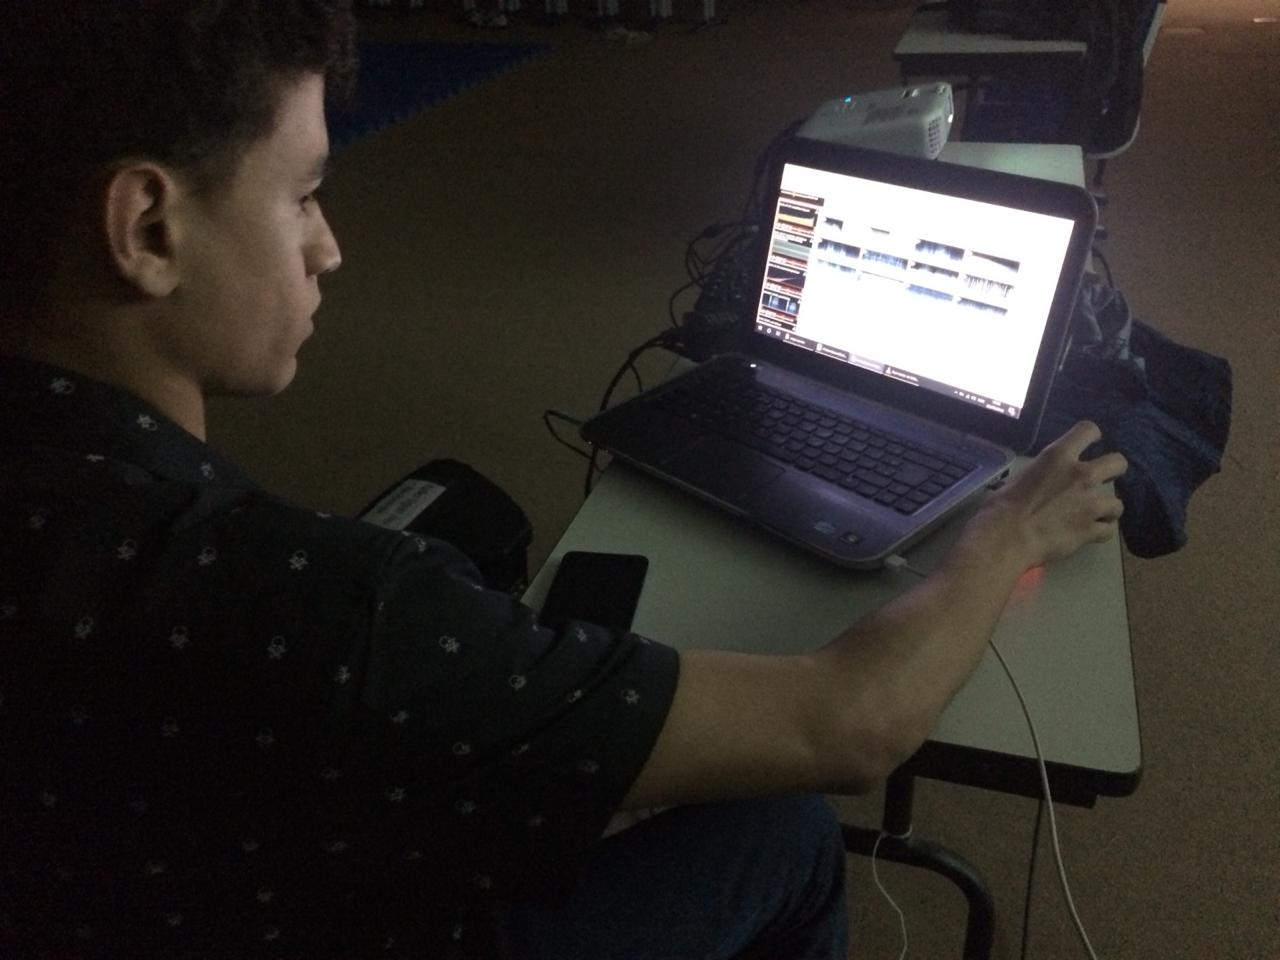
\includegraphics[width=1\textwidth]{pictures/cap4/heitor_ufsb}
\caption{\label{psufsb2}Heictor Miranda Cruz improvisando sobre a playlist pré definida pelo professor durante o exercício.}
\label{fig:psufsb2}
\end{figure}

\subsubsection{Sarau do Binho}

Já no Brasil também, pude utilizar a ferramenta durante um evento organizado pela professora Cinara Araújo no Centro de Cultura da cidade de Porto Seguro. O evento tinha como proposta ser uma edição do ``Sarau do Binho'', que acontece regularmente na cidade de São Paulo, aproveitando a presença do poeta Binho, que estava de passagem pela Bahia. Durante o evento, utilizei a ferramenta para criar paisagens sonoras sobre as quais os participantes declamaram poemas de sua própria escolha ou autoria. A ferramenta se mostrou versátil para auxiliar a composição de diferentes ambientações sonoras que puderam acompanhar temas diversos dos oemas declamados no evento \footnote{Os sons utilizados na apresentação podem ser acessados no endereço: \url{http://www.playsound.space/sounds=376415,419165,346105,320306,213318,4832,321030,125346,101195,52502,52499,84715,59356,166709,238689,396268}}.


\subsubsection{Cannibal Soundscapes}
Cannibal Soundscapes foi uma performance apresentada no Congresso UBIMUS de 2018. A proposta da performance era de produzir uma interpretação sonora do Manifesto Antropófago de Oswald de Andrade, \footnote{\cite{Andrade1928}}. Publicado em 1928 no primeiro número da ``Revista de Antropofagia'', o manifesto é considerado  marco teórico central do movimento antropofágico no Brasil.

O texto carrega referências diversas a teorias e autores, desde o pensamento revolucionário de Marx (1818- 1883), à idéia Freudiana de ``totem e tabu'', autores surrealistas como André Breton (1896 - 1966) e filósofos como Jean Jacques Rousseau (1712 - 1778), Francis Picabia (1879 - 1953) entre referências a figuras e movimentos da história brasileira. O manifesto traz a idéia de uma ``revolução Caraíba'', ``A unificação de todas as revoltas eficazes na direção do homem''. O antropófago é usado como uma metáfora para a devoração e digestão das influências culturais importadas, que deveriam ser repensadas criticamente sob os termos das condições locais \footnote{\cite{Berg-1999}}.

Para tanto, o manifesto se volta para a cultura indígena, nos lembrando que ``Já tínhamos o comunismo'' \footnote{\cite{Bradley2007}}, e se opondo a uma série de ``verdades'' trazidas junto com as caravelas que nos colonizaram. Propõe como horizonte utópico o ``matriarcado de Pindorama'', onde ``a alegria é a prova dos nove'':

\begin{citacao}
Contra a realidade social, vestida e opressora, cadastrada por Freud - a realidade sem complexos, sem loucura, sem prostituições e sem penitenciárias do matriarcado de Pindorama. \footnote{\cite{Andrade1928}}
\end{citacao}

\begin{figure}

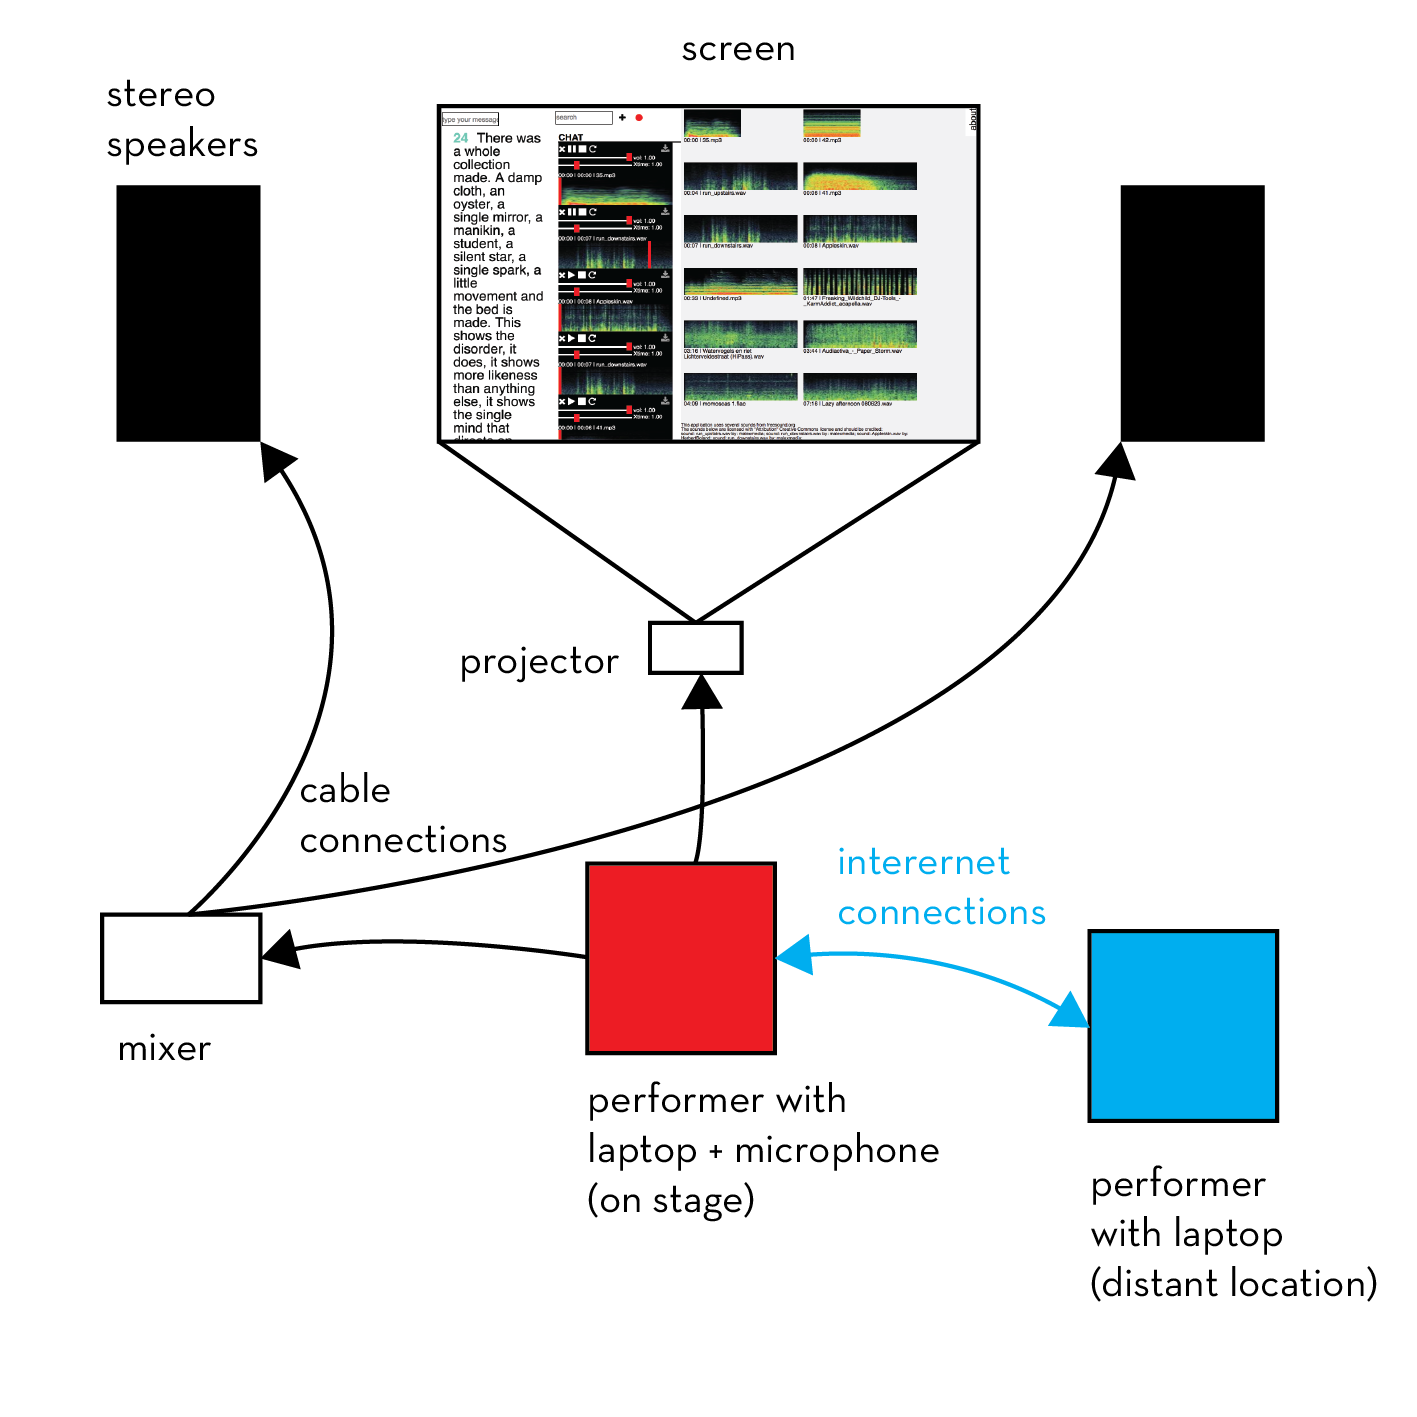
\includegraphics[width=1\linewidth]{pictures/cap4/diagrama-cannibal}
\caption{Diagrama para organização da performance no palco.}
\label{diagram}
\end{figure}

Por ser construído a partir de muitas referências da cultura brasileira, o Manifesto é um texto considerado difícil de traduzir \footnote{\cite{Lesli-1991}}. Para a performance, propusemos usar o texto original em português, e usar o sistema embutido de tradução como base para buscar as palavras no Freesound. Propusemos a performance como uma forma de aplicar também o sistema de chat que está sendo desenvolvido na plataforma. Nossa idéia era de simular um diálogo entre os dois performers, usando o texto de Oswald como base. Mathieu Barthet ia colando trechos do texto na tela, enquanto eu selecionava palavras e sons em tempo real, num processo de tradução intersemiótica \footnote{\cite{JulioPlaza1969}} mediada pelo sistema. 

A peça foi apresentada na sessão de concertos do Congresso UBIMUS, em São João Del Rey. A organização do evento não conseguiu garantir internet de boa qualidade no local do evento, então o processamento pelo sistema foi muito mais lento do que esperávamos. Apesar de ter sido possível realizar a performance proposta, a instabilidade da rede, que caiu várias vezes durante a performance causou um problema com o audio buffer, que a partir de um determinado momento, manteve um som em loop que não podia mais ser desligado.

A dificuldade em tocar sons longos no fez também rever a escolha da mudança de HTM5 para WebAudio, e para a próxima versão do software, queremos fazer uma versão mista, onde sons curtos sejam carregados no buffer e sons longos sejam tocados como objetos HTML. A experiência demontrou no entanto, as capacidades de composição em tempo real com texturas concretas, como podemos ver no espectrograma abaixo, nas figuras \ref{spceubimus} e \ref{spceubimusdt}:

\begin{figure}

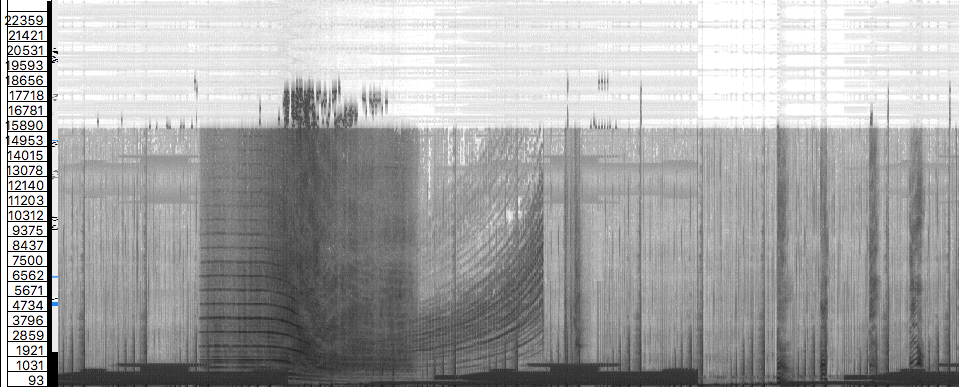
\includegraphics[width=1\linewidth]{pictures/cap4/canibalspecdbv}
\caption{Espectrograma da gravação da performance no UBIMUS.}
\label{specubimus}
\end{figure}

\begin{figure}

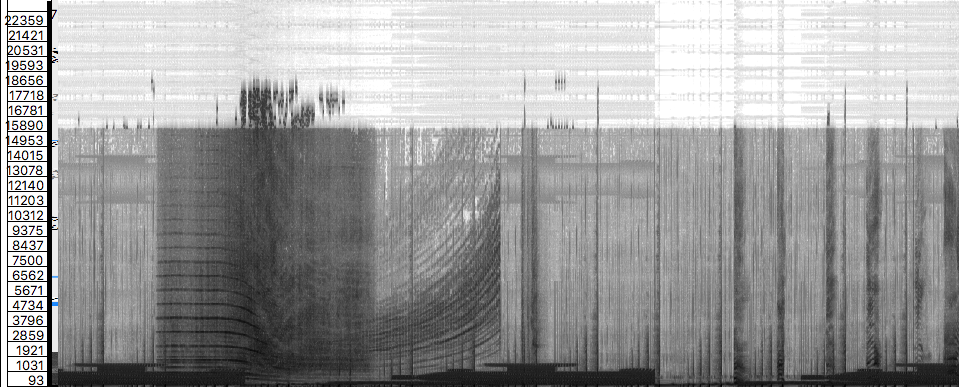
\includegraphics[width=1\linewidth]{pictures/cap4/canibalspecdbvdt}
\caption{Espectrograma da gravação da performance no UBIMUS.}
\label{spceubimusdt}
\end{figure}

\subsubsection{Tender Buttons | Sound Space}
Similar à performance anterior, onde usamos como base um texto para criar uma paisagem sonora, ``Tender Buttons | Sound | Space''  foi uma performance baseada no texto da Gertrude Stein ``Tender Buttons''\footnote{\cite{Stein1914}}. Escrito em 1914, o poema traz combinações não usuais de palavras, que está associado com uma ideia de ``destruição da sintaxe''\footnote{\cite{Perloff1996}}, que também subverte a fala e a prosa feminina tradicional\footnote{\cite{Murphy1991}}. O texto pode ser considerado como uma experiência de Stein com a liguagem, e é uma mistura de poesia e prosa com sentenças que a primeira vista podem parecer ``nonsense'', mas que ganham sentido à medida que se observa a forma que são empregadas\footnote{\cite{Perloff1996}}. Apesar de certas polêmicas a respeito da posição que a poeta veio defender na Segunda Guerra\footnote{\cite{Bernstein2012}}, que foi motivo de discussão entre a equipe, decidimos trabalhar com o poema por ser um dos poucos exemplos de prosa poética escrito por uma mulher livre de direitos autorais da Era moderna.

O texto é estruturado em três partes: \textit{Objects}, \textit{Food} e \textit{Rooms}. Nós escolhemos trabalhar com a terceira parte do poema, \textit{Rooms}, pela quantidade de sugestões sonoras que poderíamos usar durante a performance, como podemos ver neste trecho:

\begin{citacao}
Currents, currents are not in the air and on the floor and in the door and behind it first. Currents do not show it plainer. This which is mastered has so thin a space to build it all that there is plenty of room and yet is it quarreling, it is not and the insistence is marked. A change is in a current and there is no habitable exercise. \footnote{\cite{Stein1914}}
\end{citacao} 

A performance foi apresentada na Web Audio Conference de 2018, em Berlim, na Alemanha, em conjunto com Alessia Milo. Diferente da anterior, onde o texto era apresentado por escrito na tela mas a performance era apenas sonora, sem elementos discursivos, construímos essa performance baseada em uma leitura que eu fiz do poema, que foram cortados, selecionados e transferidos para o banco de dados do Freesound. Desta forma pudemos tocar esses trechos durante a performance e criar a paisagem sonora por cima das leituras. Assim, enquanto Alessia soltava os trechos da leitura, e colava o texto na janela do chat, eu ia selecionando os sons e tocando com eles. 

Pelas condições de som e internet no local, que eram excelentes, considero que essa performance foi mais bem sucedida que anterior, já que não houveram bugs e os sons foram carregados rápidamente. Em um momento, por volta da metade da performance, quando abri uma quantidade de sons considerável, senti que o sistema começou a ficar um pouco lento. Foi apenas remover alguns dos sons que já estavam carregados que a performance continou correndo normalmente. Um vídeo da performance, que durou 20 minutos está dispoível em: \url{https://www.youtube.com/watch?v=LiNb_T8oluA}

\begin{figure}

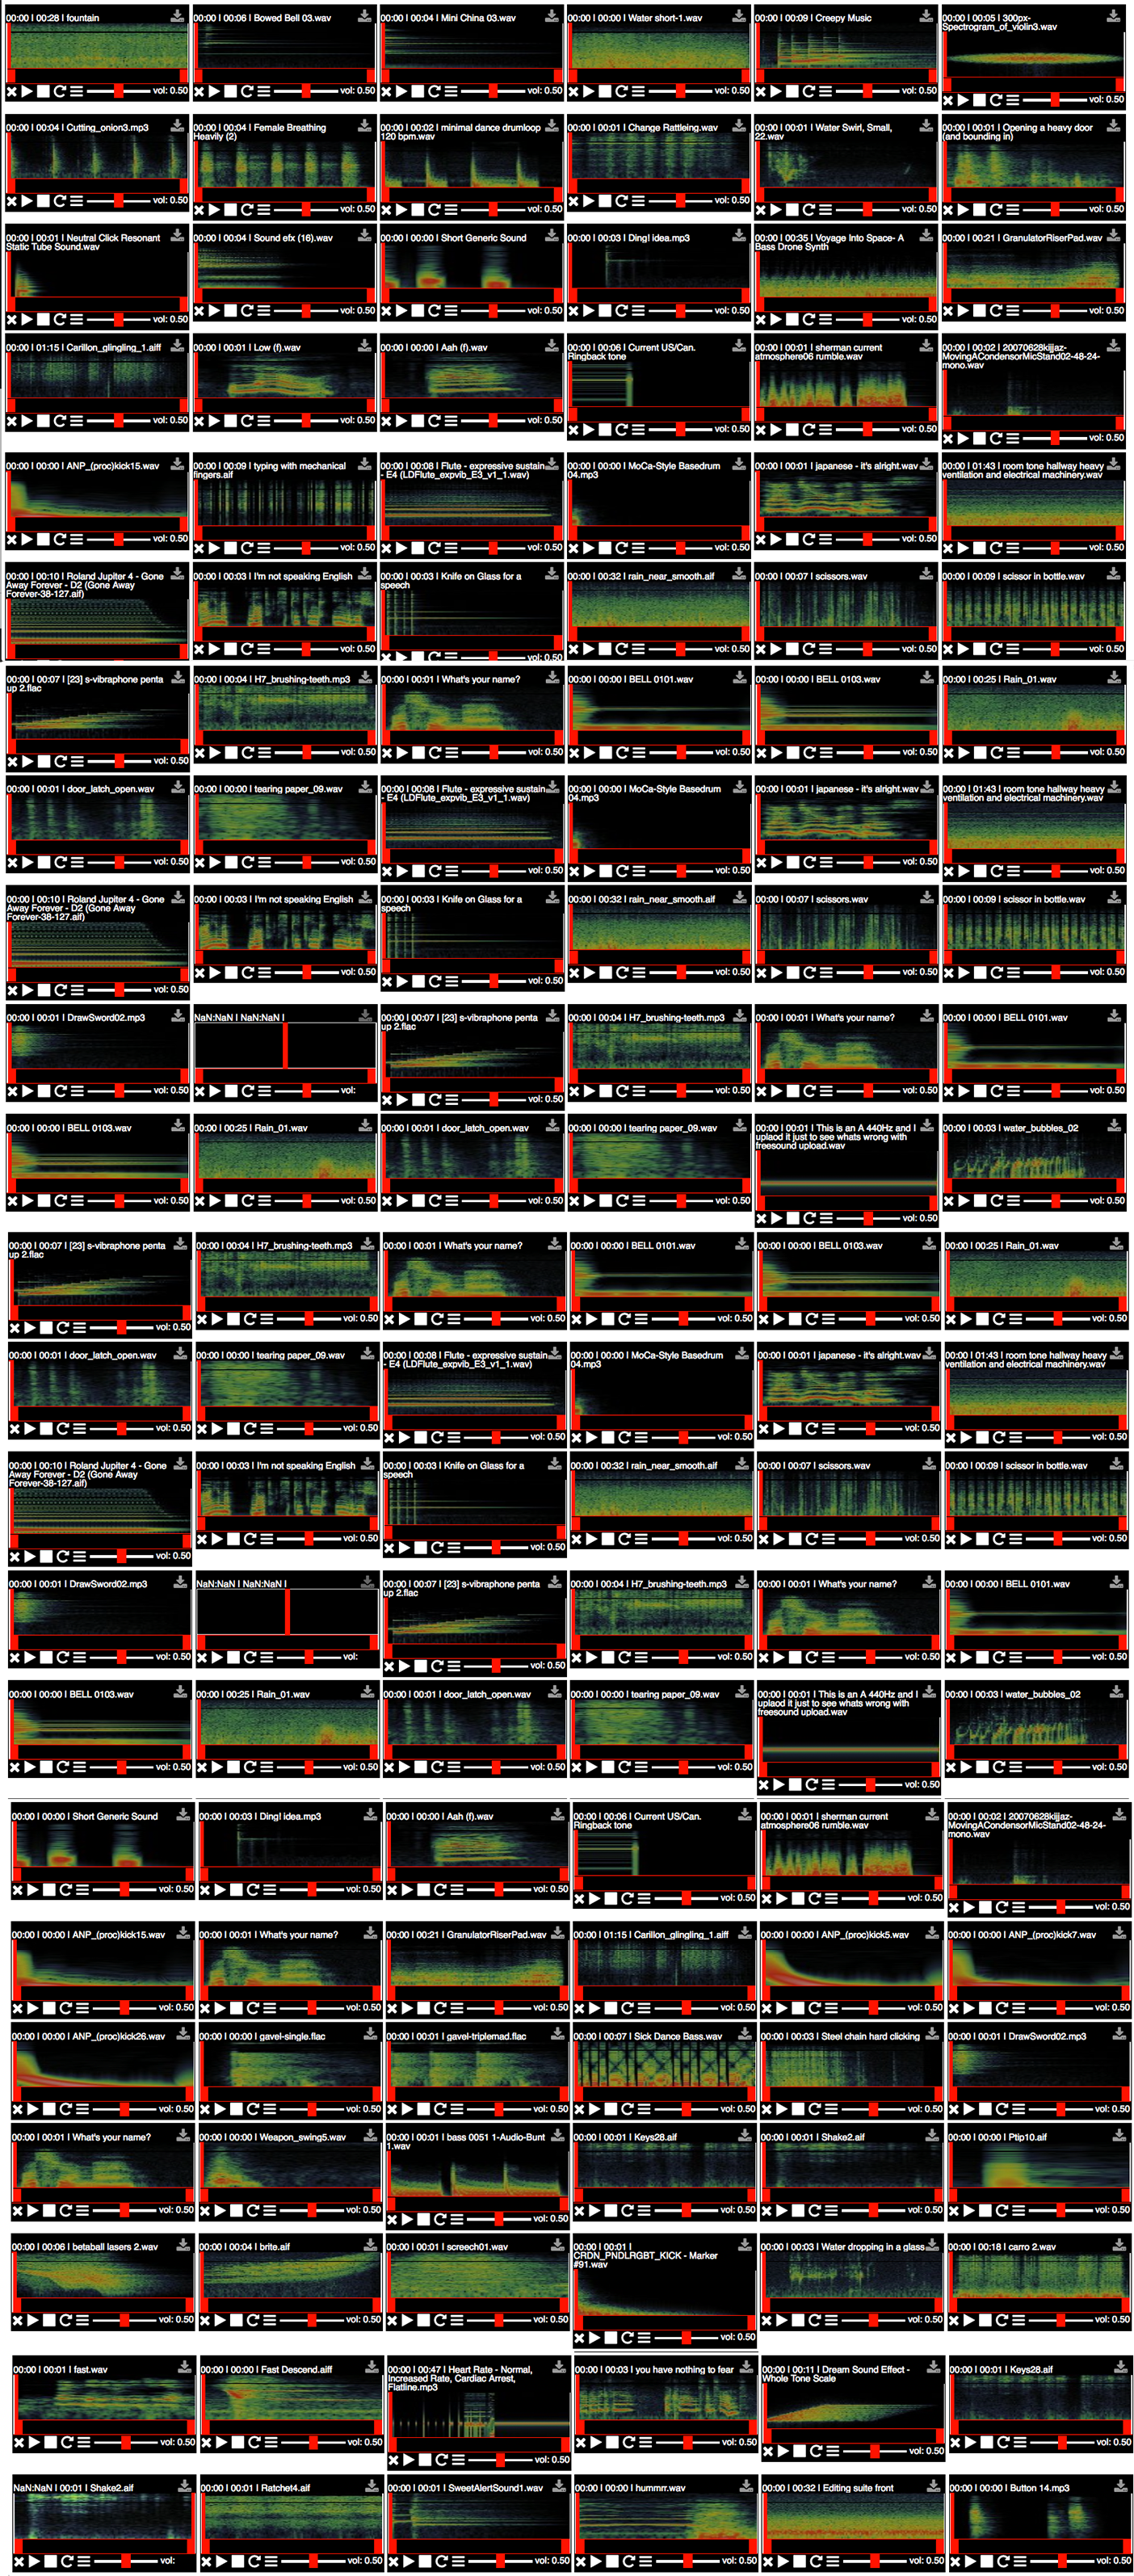
\includegraphics[width=0.8\linewidth]{pictures/cap4/tenderbuttonssounds}
\caption{Todos sons utilizados na performance.}
\label{diagram}
\end{figure}




\subsubsection{Imagina! Reverbera}

No meu segundo quadrimestre de trabalho na UFSB, ministrei o componente ``Oficina de prática em criação sonora'', onde trabalhamos processos de improvisação musical. Recebemos o convite da professora Juliana Gontijo para realizar uma sessão especial do projeto Imagina!, que realiza projeções de cinema em diversas sessões no município fazendo a sonorização ao vivo de filmes mudos. para a primeira sessão, selecionamos três filmes mudos para improvisar coletivamente sobre eles, criando uma trilha sonora ao vivo. A performance contou com a participação dos quatro alunos da turma: Gislania Araújo, Heictor Miranda Cruz, Herverton Taua Silva dos Santos e Marilucia Moreira, todos eles estreantes em performance ao vivo e iniciantes em práticas de improvisação musical, e dois outros alunos que já eram músicos, Eduardo Rebelo da Silva e Ítalo Rodrigues, que se juntaram pelo interesse no projeto.
\begin{figure}

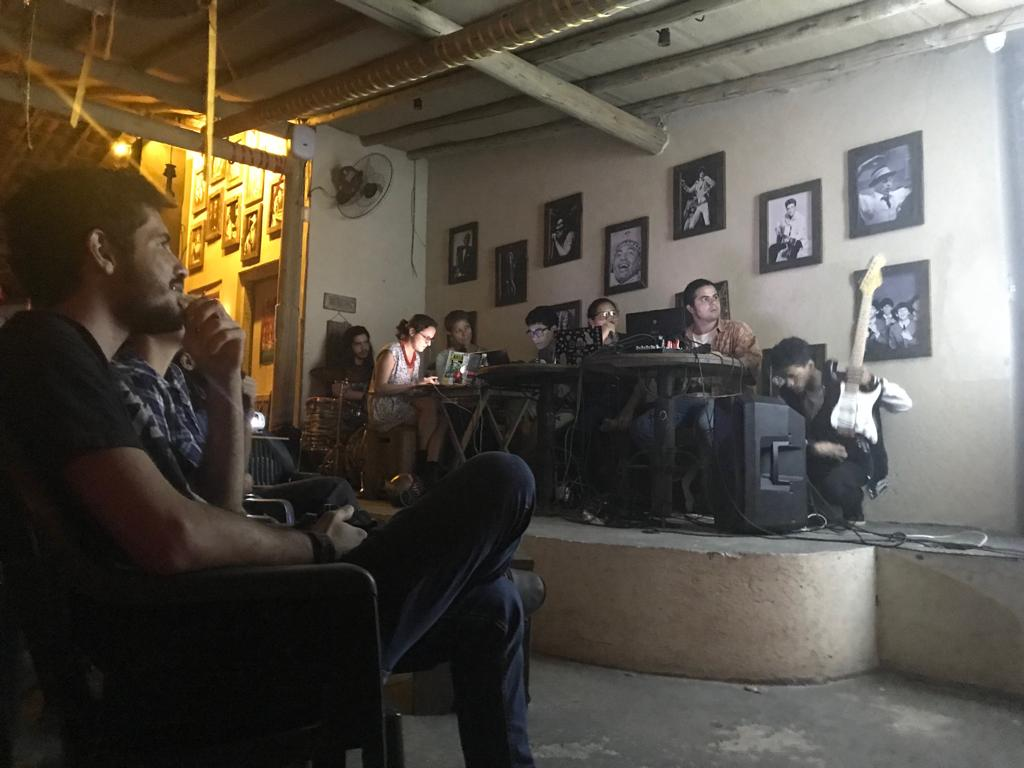
\includegraphics[width=0.7\linewidth]{pictures/cap4/imagina1a}
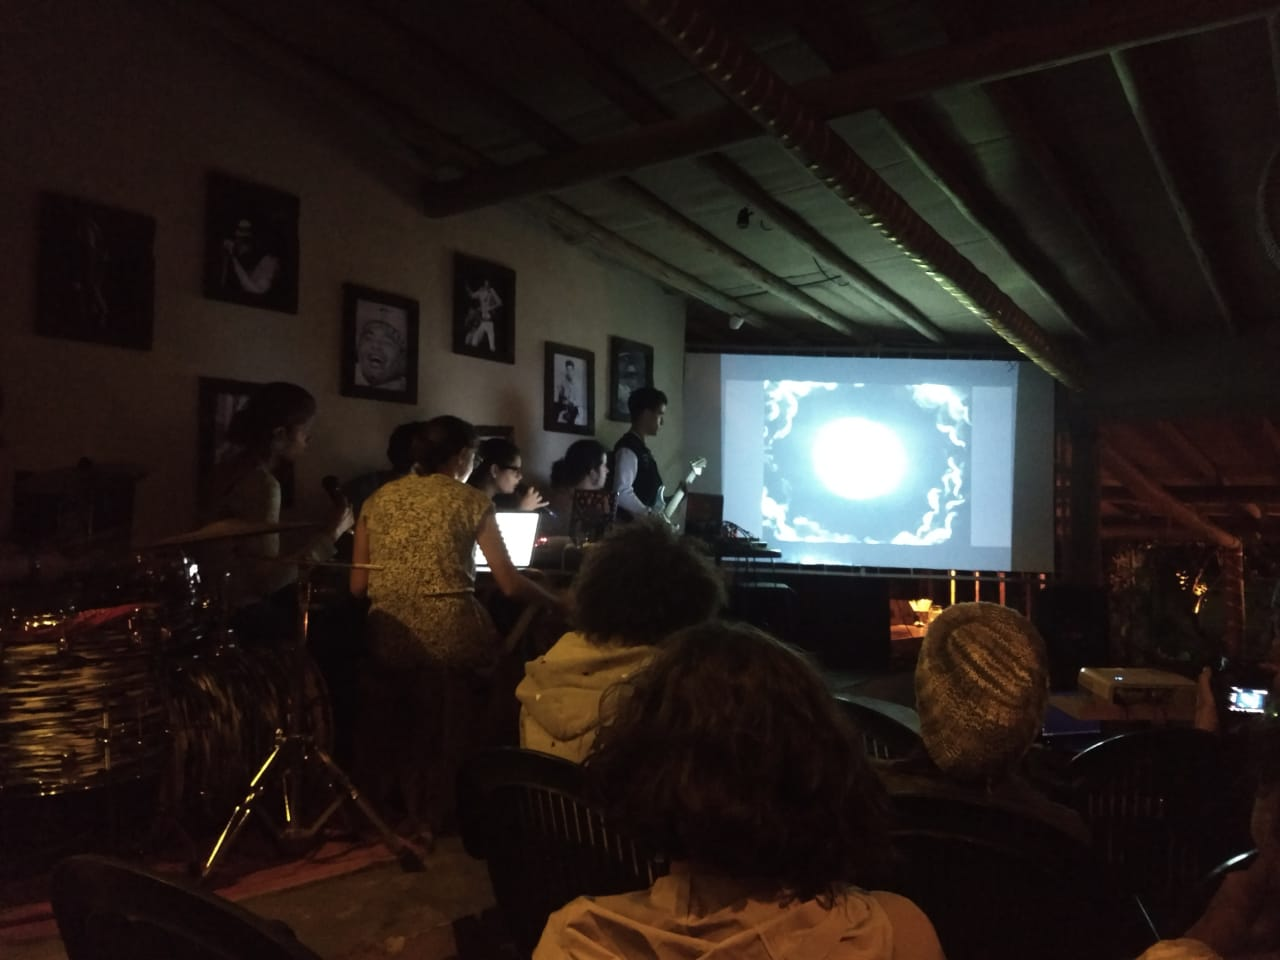
\includegraphics[width=0.7\linewidth]{pictures/cap4/imagina1b}
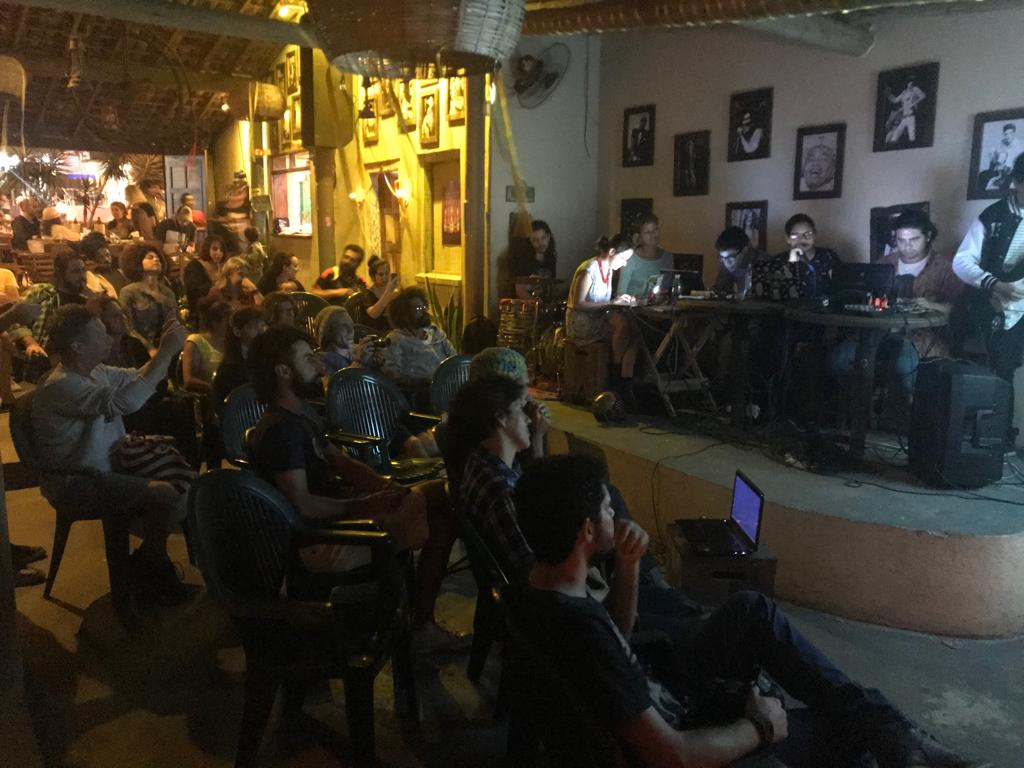
\includegraphics[width=0.7\linewidth]{pictures/cap4/imagina1c}
\caption{Imagina! Reverbera.}
\label{Fotos: Juliana Gontijo}
\label{diagram}
\end{figure}


Na ocasião, eu e a aluna Gislânia usamos PS como ferramenta para tocar, em conjunto com instrumentos de percussão e voz. Os outros participantes tocaram com seus instrumentos tradicionais (computador, guitarra, bateria, voz, percussão). Como não sabíamos as condições de internet no local, decidimos trabalhar com sons pré-selecionados, como um roteiro para garantir que o sistema funcionasse mesmo sem internet, apesar de necessitar de internet para a busca de sons, o sistema funciona mesmo offline. Uma vez que os sons são carregados no buffer, é só manter a página aberta que podemos tocar com a ferramenta normalmente.

Para acompanhar os filmes, preparamos as seguintes playlists: 

\url{http://www.playsound.space/sounds=373811,36274,50737,360540,398712,238454,423526,397948,145685,47623,76420,76421,397948,417046,76422,435415,435414,340646,238456,238452,162761,264538,191240,274354}

\url{http://www.playsound.space/sounds=245381,394898,320303,24338,372181,411206,379249,266977,266916,382735,331624,321404,193900,188048,188051,373751,193810,193808,369913,433584,416439,7454,134968,101871,220910,326542,341561,411521,348519,378211,50820,50823}

Para tocar, utilizamos sons concretos, que tinham relação com as imagens apresentadas, como sons de mar, floresta, trânsito, bicicleta, e sons musicais para criar atmosferas de festa, ou de suspense dependendo do filme. Os sons tocados através da ferramenta funcionaram em grande parte como uma textura de base para os demais músicos improvisarem, garantindo um fluxo sonoro constante que ajudou a dar segurança ao demais participantes, que eram aprendizes na prática de improvisação livre.





\subsubsection{Transmusiking II}

Na semana do dia 20 de novembro de 2018, o grupo Female Laptop Orchestra, do qual também faço parte desde a conferência Audio Mostly de 2017, quando participei da performance da peça Transmusiking com o projeto Banda Aberta, participou de uma residência no Sonic Arts Research Institute (SARC) da Queen's University em Belfast. Devido ãs atividades de docência e pesquisa em andamento e à distância e os custos de transporte, pude participar apenas remotamente do processo, que contou com a participação das musicistas residentes Nela Brown (Londres, Inglaterra), Anna Xambo (Trondheim, Noruega), Magdalena Chudy (Warsaw, Polônia), Tuna Pase (Barcelona, Espanha), Liz Dobson (Huddersfield, UK), Ada Mathea Hoel (NTNU Norway) e Franziska Schroeder (Belfast, UK) e colaboração à distância de Sonia Wilkie (Melbourne, Austrália) e Lea Ikkache (Paris, França) além da minha, por streaming do Brasil. O projeto se propôs a realizar um painel sobre a participação das mulheres no campo da tecnologia musical ao redor do mundo e um concerto coletivo, para o qual propusemos uma nova versão da peça Transmusiking:


\begin{citacao}
Transmusicking II continues to explore geographical, cultural, technical and artistic challenges of collaborative music making, with co-located and distributed musicians who use multiple tools to relay musical information and create music together. This collaboration draws on the experience gained from Transmusicking I, premiered at Audio Mostly 2017, London.

As remote performers, despite real-time connectivity, we often experience a sense of loneliness. For this performance, we focus on the sense of “togetherness” by re-uniting musicians who come from distinct cultural backgrounds with different instruments and technologies. 

Distributed performers will use SARC’s mobile phone app liveSHOUT to send audio streams of cello, flute and live coding to the web-based Locus Sonus platform. Co-located musicians will improvise using saxophone, environmental loops and online sound libraries. 
The mix of the incoming streams and the onsite performers’ inputs will be spatialized into the performance space.

Live visuals will be produced to reinforce the themes of latency, collaboration, and togetherness. (email enviado por Magdalena Chudy à direção do SARC)
\end{citacao}

Durante a residência as participantes produziram uma partitura para organizar a participação das demais envolvidas no processo:

\begin{citacao}


SARC Concert

Each piece is approx. 10 minutes

To streamers: When you are streaming, don’t forget that you are solo during the first minute, so it will be good to play all your material and after the first minute you can take rests. 



1. Sonia streaming (Melbourne) 
1- 1 minute of  Sonia Streaming solo, Ada can take her stream and move here around the space. 
2-  Nela comes in with her 3D Belfast soundscape and Liz LFO. 
3-  We start duets as is we are cars passing by or people around. 
    1st duet Magda \& Ada- 2-3 minutes Ada 
    2nd duet Tuna (vox) \& Anna -2-3 minutes 
4- Sonia \& Nela with soundscapes.- Ada plays rhythmic and she stays solo at the end and fades out. 


2. Ariane streaming (São Paulo) 
1- 1 minute of  Ariane streaming solo, Ada can take her stream and move it around the space. (Ariane uses vocal, piano and soundscape of water)
2- Vive/Sax \& Liz duo - 5 minutes 
Ariane if you send piano play F,G,A
3- Voice duet  Ada \& Ariane- 2 minutes 
4- Play all breathy and watery  and Tuna (Wasserbass) fades out with water instrument - 1 minute   

3. Lea streaming (Paris) The drone piece and Tutti 
1- 1 minute of  Lea streaming solo, Ada can take her stream and move it around the space. 
2- 4 minute done build up (Tuna-Dronetext)
3- Flute que for the glitch/stacatto part to start and stop
Liz wobbles with the others. 
4- Stop and Rest!
5- Magda brings the drone back.
6- Fade out the drone until Lea’s singing bowl comes back. 
\end{citacao}

Para viabilizar a execução da peça, organizamos alguns ensaios via skype, onde testamos o setup no computador e o feedback recebido das performers que estavam em Belfast. Na minha participação no concerto, utilizei técnicas vocais expandidas para improvisar sobre uma base preparada no PS, onde selecionei sons de piano, de água e um sino invertido. 

Para fazer o \emph{streaming}, utilizei um aplicativo chamado Butt (Broadcast using this tool) que é um servidor alternativo de Icecast para windows e mac, utilizando o servidor \url{http://crowdj.net/}. Para enviar em conjunto o som que vinha do navegador e o som do microfone, foi preciso instalar um servidor de áudio que unia os fluxos sonoros de diferentes fontes do sistema. O atraso do som durante a transmissão era de cerca de sete segundos, e eu recebia o feedback das performance através do skype. Para não re-alimentar o som enviado com a resposta, o som era recebido da Irlanda pelo celular, enquanto eu tocava com o computador, o que me obrigou a usar dois fones de ouvido sobrepostos, para evitar vazamentos de áudio para o microfone. Apesar da logística complexa, a performance foi bem sucedida, devido a estratégias de tocar que não dependessem de um retorno imediato. Procurei produzir principalmente texturas, e por ser a fonte externa durante a parte da peça que toquei, acabava sendo um guia que enviava o som, enquanto as performers que estavam no local respondiam ao que eu enviava. 


Separei uma seleção de sons de piano: 


http://www.playsound.space/sounds=386440,351623,339821,316025,148571,176494,396483,427086,134908,332114,432441,232131,356107,373906,355826,355979,296145,148505,148508,409480,176494,351324,148548,295857,448552,148510,176504,351327,320306,320311,371494

\begin{figure}


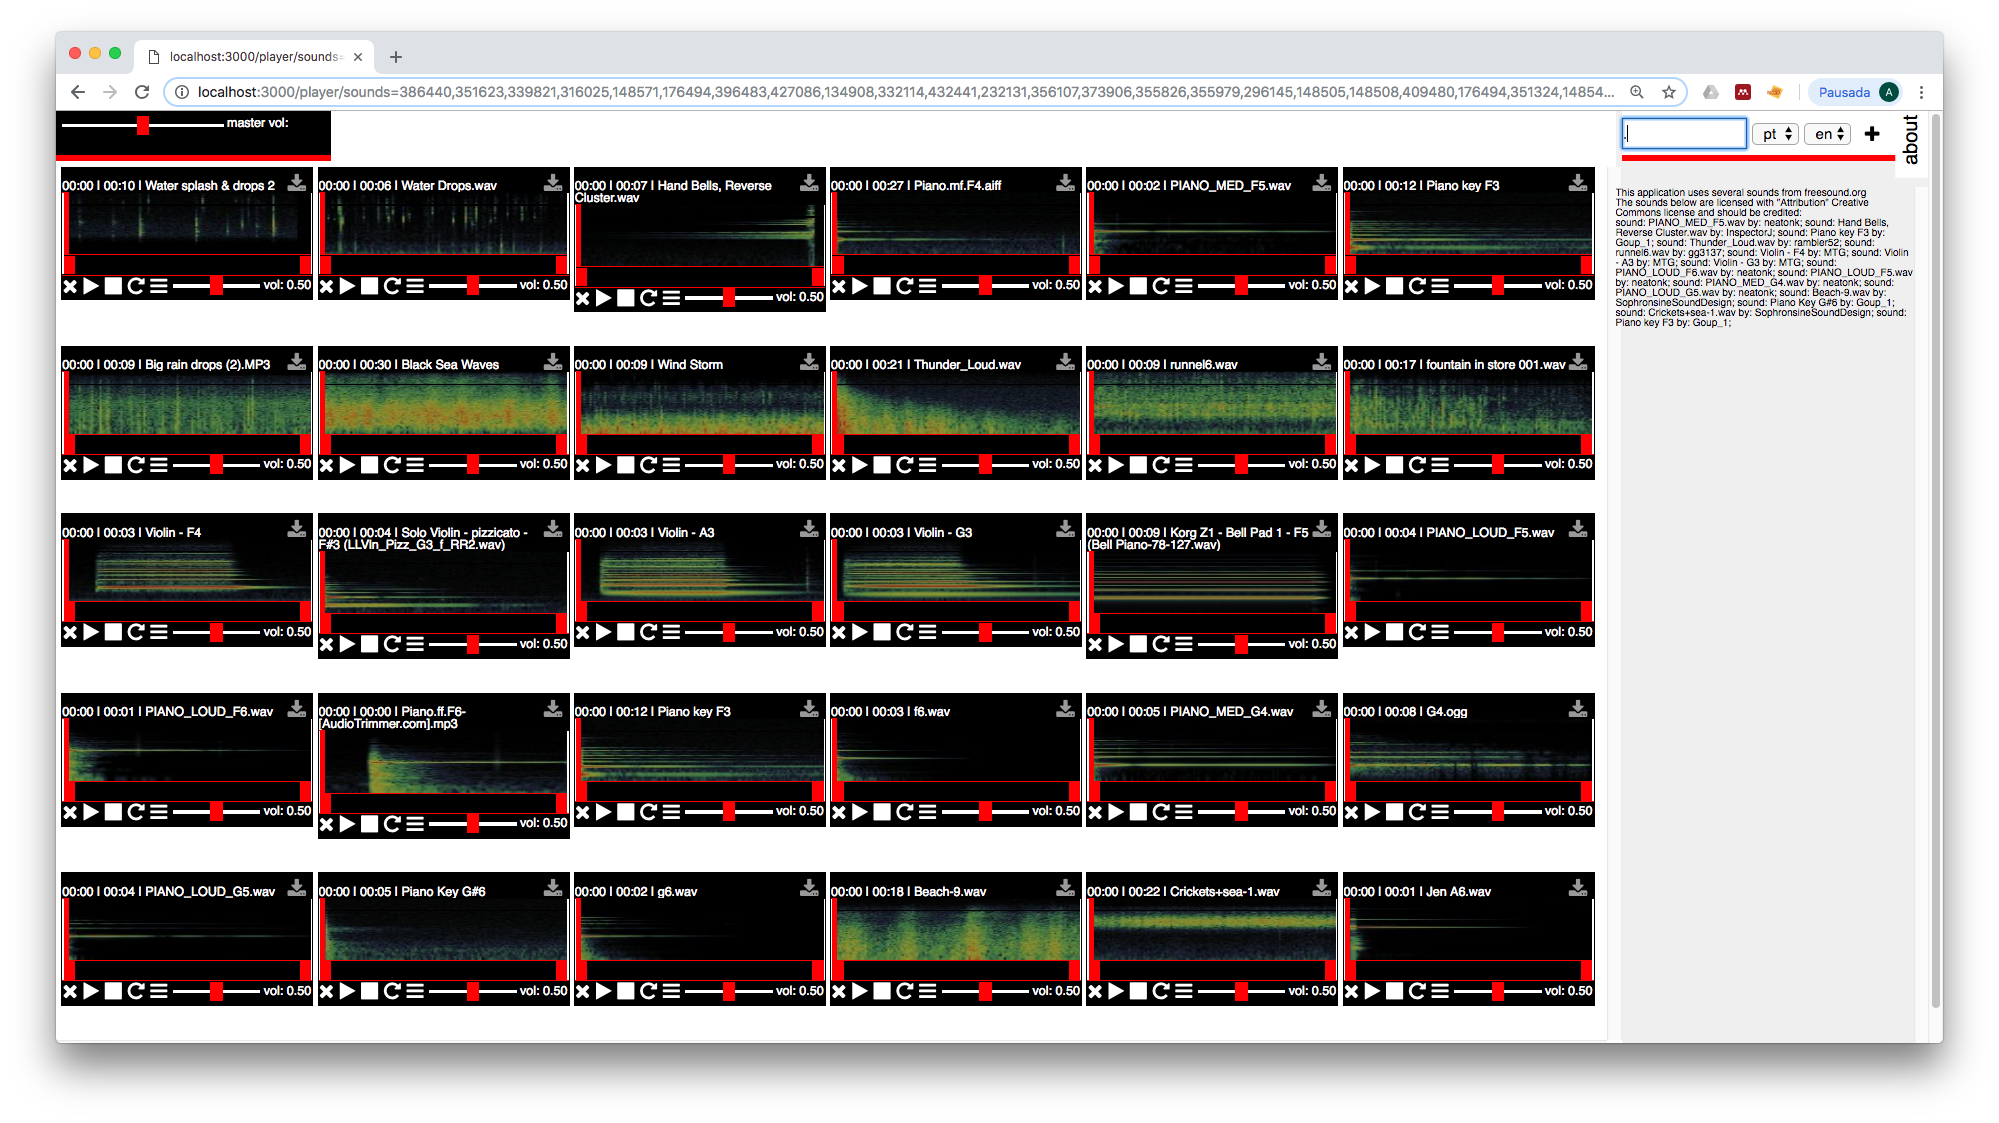
\includegraphics[width=0.7\linewidth]{pictures/cap4/playsound_sarc}
\caption{Sons usados na performance com a FLO.}
\label{telasarc}
\end{figure}

sons usados:

\url{http://www.playsound.space/sounds=386440,351623,339821,316025,148571,176494,396483,427086,232131,296145,148505,148508,409480,176504,351327}

sound: Hand Bells, Reverse Cluster.wav by: InspectorJ; sound: PIANO\_MED\_F5.wav by: neatonk; sound: Piano key F3 by: Goup\_1; sound: PIANO\_LOUD\_F5.wav by: neatonk; sound: PIANO\_LOUD\_F6.wav by: neatonk; sound: Piano Key G\#6 by: Goup\_1;

\begin{figure}


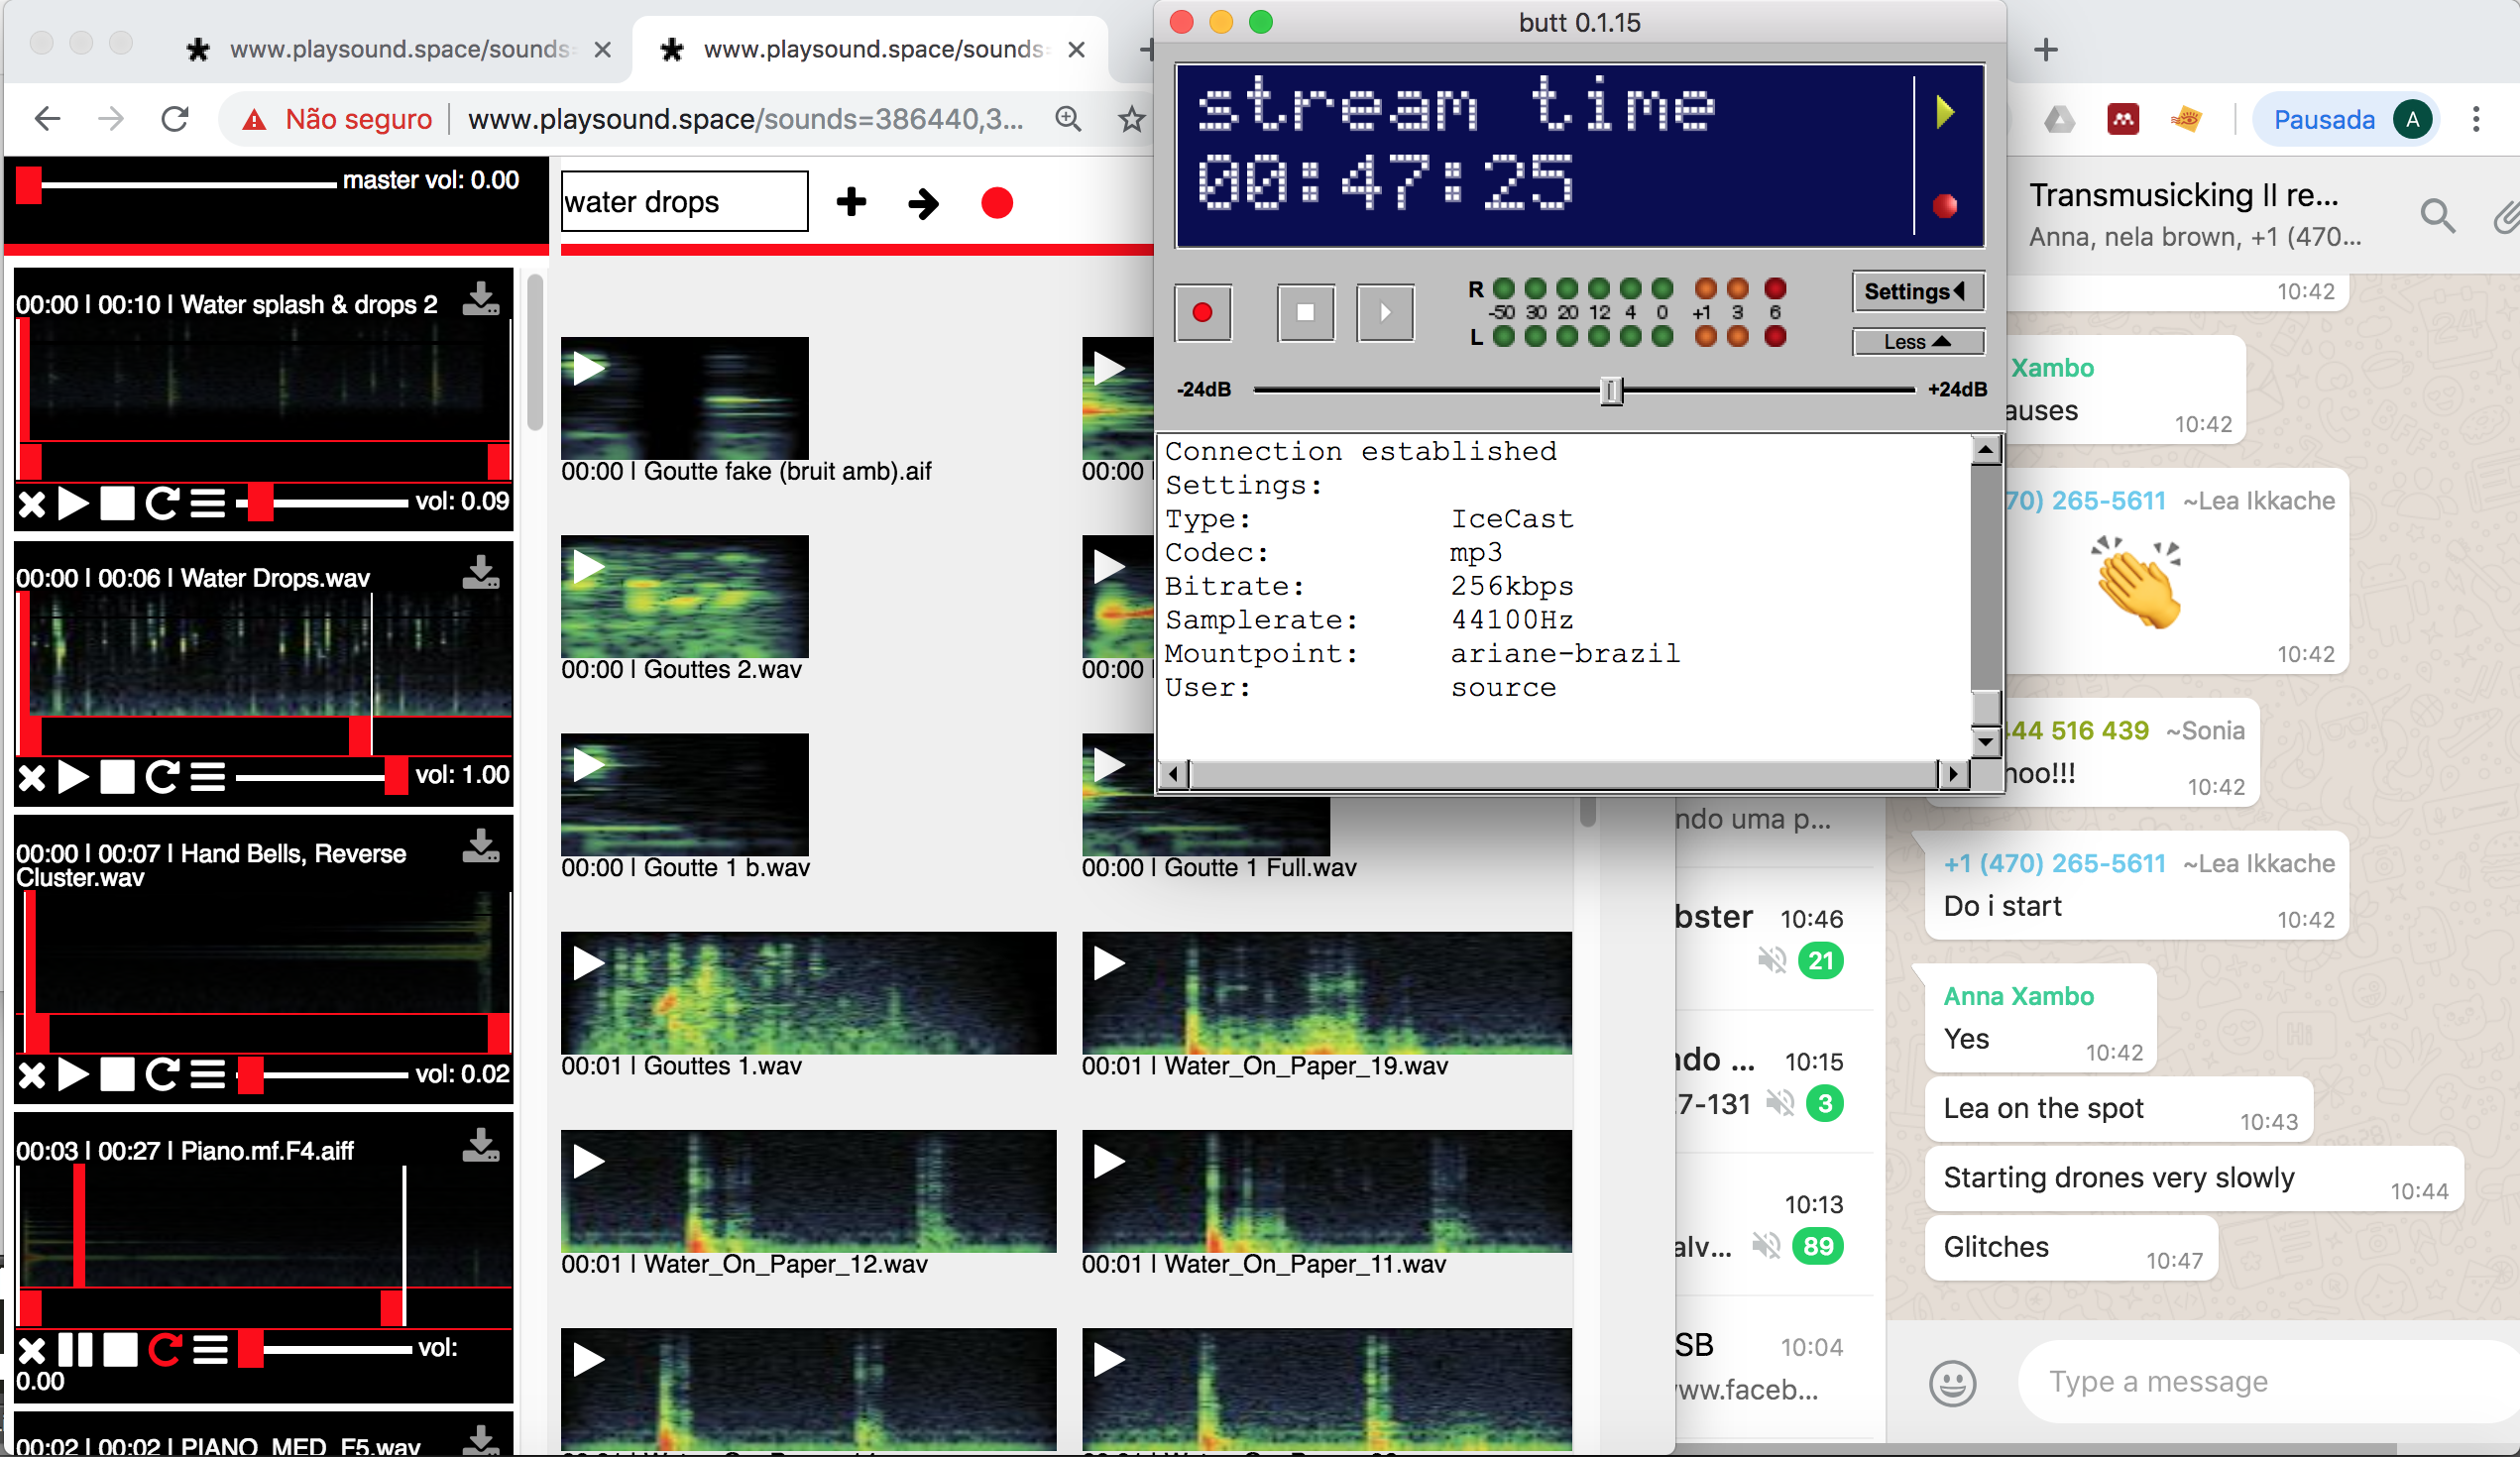
\includegraphics[width=0.7\linewidth]{pictures/cap4/telasarc}
\caption{Screenshot da tela no momento da apresentação online, com Playsound, Butt, para streaming e whatsapp para comunicação com o grupo à distância.}
\label{telasarc}
\end{figure}



\phantomsection



The Fall of the House of Usher  - 13 min - Melville Webber (1928)
\url{https://www.youtube.com/watch?v=mxjCWleWXf4}

Spook Sport - 8 min - Mary Ellen Bute (1940)
\url{http://www.ubu.com/film/bute_spook.html}

The Life and Death of 9413: A Hollywood Extra - 13  min - Slavko Vorkapich \& Robert Florey (1928)
\url{https://www.youtube.com/watch?v=b3M5znXDlm4}

The cameraman' s revenge  - 13 min - Ladislaw Starewicz (1912)
\url{https://www.youtube.com/watch?v=Q9lUcKtPTYY&feature=youtu.be}




